\chapter{Theoretical and phenomenological background}
\label{ch:background}
\graphicspath{{Chapter-Background/figures/}}

\section{Quantum chromodynamics}
\subsection{History and experimental motivation}

The atomic nucleus was discovered in the early 20th century \cite{Rutherford:1911zz}, and a few years later it was determined that it was composed of protons ($p$).
An additional, electrically-neutral nuclear constituent particle was proposed soon after and the neutron ($n$) was finally discovered in the early 1930s \cite{Chadwick:1932ma}.
This indicated that there was some new type of interaction strong enough to overcome electrostatic repulsion between protons that binds nucleons ($p$ and $n$) together in the nucleus.
A particle field, the pion ($\pi^\pm$, $\pi^0$), was proposed to mediate this strong interaction \cite{Yukawa:1935xg}.
Since the strong interaction only acts over a length scale of about 2 fm, the mediating pion was predicted to have a mass of about 100 \MeV\footnote{The potential mediated by a boson of mass $m$ is proportional to \( - \exp(-mcr/\hbar)/r\), where $r$ is the separation between a pair of participants. Thus the mass of a mediating boson for a potential with a characteristic cutoff length of $\lambda$ is $m = \hbar/c\lambda = \frac{200 \MeVcc \textrm{fm}}{\lambda}$.}.
The charged pion was indeed discovered experimentally in 1947 \cite{Lattes:1947mw}.
Pions can be interpreted as the Nambu-Goldstone bosons corresponding to the spontaneously broken chiral symmetry, which explains their relatively small masses.

The expanding body of observed hadrons --- particles bound by the strong nuclear interaction --- and the allowed decays thereof suggested additional conserved quantum numbers and that they could be composed of constituent particles.
It was noticed that hadrons can be organized by their quantum numbers in a manner described by an $SU(3)$ \emph{flavor} symmetry \cite{GellMann:1962xb}.
This suggests that hadrons are composed of constituent particles called \emph{quarks}, each with a quantum number called flavor that can takes a value of ``up'' ($u$), ``down'' ($d$), or ``strange'' ($s$)\footnote{Three heavy flavors have since been discovered, ``charm'' ($c$), ``bottom'' ($b$), and ``top'' ($t$), but heavy quarks and the hadrons composed of them decay very rapidly due to their larger mass.}.
The quark model was not immediately accepted because free quarks were not (and still have not been) observed.
Scattering experiments were needed to probe the internal structure of hadrons.

Because electrons are point-like particles to the limits of current experiments, a scattering process $e^- A \rightarrow e^- X$ is dependent only on the internal structure of the target $A$.
The electron scatters through a virtual photon that interacts directly with the hadron in a process called \ac{DIS}\footnote{``deep'' in that it probes the constituent structure of the target and ``inelastic'' because kinetic energy and matter are exchanged in the creation of the product particles}.
The kinematics of the electron in this type of experiment constrain the structure of the target hadrons.

\begin{figure}[t]
  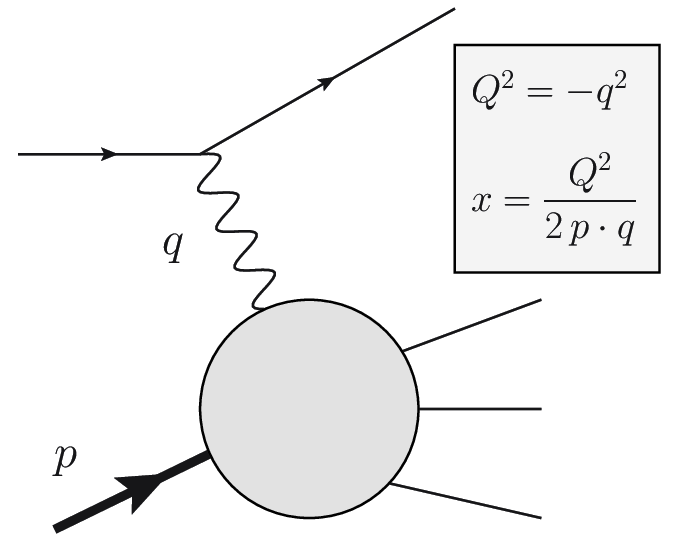
\includegraphics{dis_electron_proton.png}
  \caption{Deep inelastic scattering of a lepton on a hadron \cite{dis_fig_proceedings}.}
  \label{fig:dis}
\end{figure}

Under the constraints of Lorentz and gauge invariance, the cross-section of an unpolarized \ac{DIS} process with incoming lepton and proton momenta $k$ and $P$ respectively and momentum transfer $q$ can be expressed as \cite{Tanabashi:2018oca}
\begin{equation}
  \frac{d^2 \sigma}{dx \, dQ^2} = \frac{4\pi\alpha^2_\textrm{EM}}{2xQ^4}\left[ \left(1+(1-y)^2\right) F_2\left(x, Q^2\right) - y^2 F_L \left(x, Q^2\right) \right]
  \label{eq:dis}
\end{equation}
where $Q^2 = -q^2$ is the absolute magnitude squared of the photon's virtuality, $y = \frac{q \cdot P}{k \cdot P}$ is the fraction of the lepton's energy lost in the nucleon's rest frame, and $x = \frac{Q^2}{2q \cdot P}$.
In the parton model, which describes the proton as approximately-free point-like quarks in the infinite longitudinal momentum frame, $x$ is interpreted as the fraction of the target proton's momentum carried by a struck parton.
The structure functions $F_i(x, Q^2)$ describe the inherent internal structure of the proton.
The longitudinal structure function $F_L = F_2 - 2xF_1$ is zero by the Callan-Gross relation \cite{Callan:1969uq}.
In experiment the ratio $2xF_1 / F_2$ is consistent with unity independent of $x$.
In the parton model, where the proton is described in terms of free point-like quark constituents, the structure function $F_2$ is decomposed into \acp{PDF}
\begin{equation}
F_2 \left(x, Q^2\right) = x \sum_q e_q^2 f_{q/p}(x)
\end{equation}
to lowest order in the strong coupling constant $\alpha_s$.
The independence of $Q^2$ of the \acp{PDF} is a manifestation of their point-like description in the parton model and is known as \emph{Bjorken scaling}.
Logarithmic corrections are understood theoretically and arise as gluon radiation from the quarks becomes relevant at small $x$ (\cref{fig:proton_f2}).

\begin{figure}[t]
  %% page 326 of particle review
  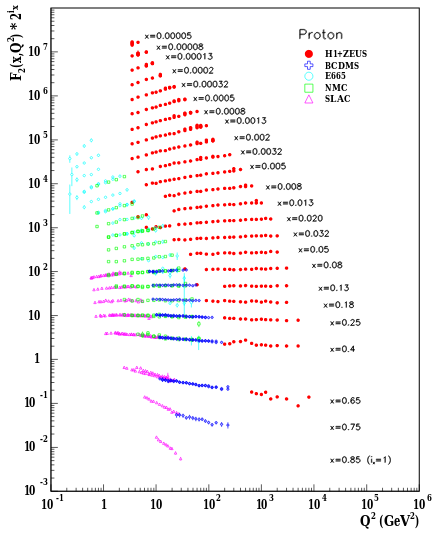
\includegraphics[width=0.45\linewidth]{proton_f2.png}
  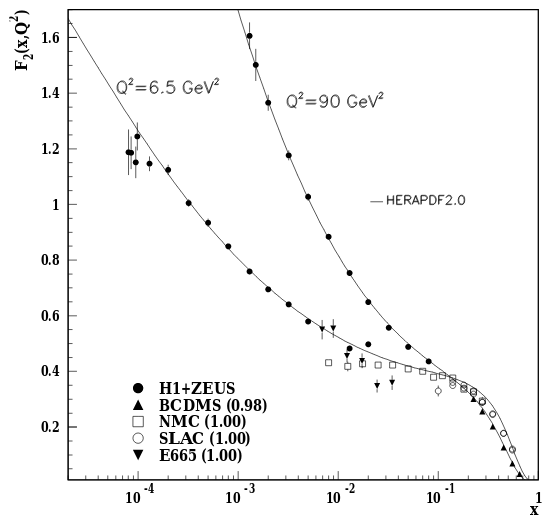
\includegraphics[width=0.54\linewidth]{proton_f2_vs_x.png}
  \caption{The structure function $F_2\left(x, Q^2\right)$ of the proton as a function of $Q^2$ (left) and of $x$ (right) \cite{Tanabashi:2018oca}.}
  \label{fig:proton_f2}
\end{figure}

An experimental and phenomenological description of the nucleon structure functions does not provide a complete description of the interactions among nucleon constituents.
The success of gauge theories in describing \ac{QED} ($U(1)$) and electroweak theory ($U(2) = SU(2) \otimes U(1)$) suggests that some other gauge theory may be able to describe the nuclear interaction.
A quantum field theory with an $SU(N_c)$ ``color'' symmetry with $N_c$ colors, called \qcd, is one such candidate.
For it to be a believable description of the strong interaction it must not only be consistent with experimental observations but also explain why free quarks have never been observed.
The rate of hadronic production in electron-positron collisions is proportional to $N_c$, so experimental measurements of the ratio\footnote{at energies above the $b\bar{b}$ threshold and below the mass of the $Z$ boson}
\begin{equation}
R \equiv \frac{\sigma\left(e^+ e^- \rightarrow \textrm{hadrons}\right)}{\sigma\left(e^+ e^- \rightarrow \mu^+ \mu^- \right)} \approx N_c \sum_{q \in \{u,d,s,c,b\}} e_q^2 = \frac{11}{9} N_c
\end{equation}
have been made to determine the number of colors, showing very good agreement with a value of $N_c = 3$.
Though the non-abelian character of \qcd makes many practical calculations difficult, it has shown remarkable success in describing the strong interaction, as will be discussed in the remainder of this section.

\subsection{The QCD Lagrangian}
The gauge-invariant lagrangian density of \qcd \cite{Wilczek:2000ih} is that of an $N_c=3$ Yang-Mills theory given by
\begin{equation}
  \Lagr_\mathrm{QCD} \equiv -\frac{1}{4} G^a_{\mu\nu}G^{a\mu\nu} + \bar{\psi} \left( i \slashed{D} - m \right) \psi \; .
\end{equation}
Here repeated indices are summed, where $\mu$ and $\nu$ indicate spacetime indices, $a$, $b$, and $c$ indicate color indices in the fundamental ($N=3$) representation, and $A$, $B$, and $C$ indicated color indices in the adjoint ($N=8$) representation.
The slash notation refers to contraction with the gamma matrices $\{\gamma^\mu, \gamma^\nu\} = 2\eta^{\mu\nu}$\footnote{with Minkowski signature $(+---)$}.
The covariant derivative is given by
\begin{equation}
  D_\mu \equiv \partial_\mu - i g A^C_\mu t^C
\end{equation}
where $A^C_\mu$ is the gluon field, $t^C$ are the generators of the $SU(3)$ gauge group, and $g$ is the strong charge constant.
The constant $g$ in the lagrangian is always squared when computing rates from quantum amplitudes, so physical results are typically expressed in terms of
\begin{equation}
  \alpha_s \equiv \frac{g^2}{4\pi} \; ,
\end{equation}
which is typically called the strong coupling constant.
The gluon field strength tensor is
\[ G^A_{\mu\nu} \equiv \partial_\mu A^A_\nu - \partial_\nu A^A_\mu + g f^{ABC} A^B_\mu A^C_\nu \]
where the $SU(3)$ structure constants $t^A$ are defined such that
\[ [t^A,t^B] = if^{ABC}t^C \; \footnote{In the $SU(2)$ gauge group the adjoint representation is three-dimensional and the structure constants are given by the anti-symmetric Levi-Civita symbol $\epsilon^{ABC}$}.\]
The quark fields are defined such that the mass matrix $m$ is diagonal:
\[ \bar{\psi}m\psi = \sum_{q = u,d,s,\ldots} m_{q}\bar{q}q \]
The quark masses $m_q$ are generated by the mechanism of spontaneous electro-weak symmetry breaking in which the Higgs field, coupling to fermions and electro-weak gauge bosons, acquires a nonzero vacuum expectation value.
This procedure induces in the \qcd vacuum a breaking of the chiral symmetry $SU(N_f) \times SU(N_f) \rarrow SU(N_f)$ in the massless Lagrangian.

\begin{figure}[t]
  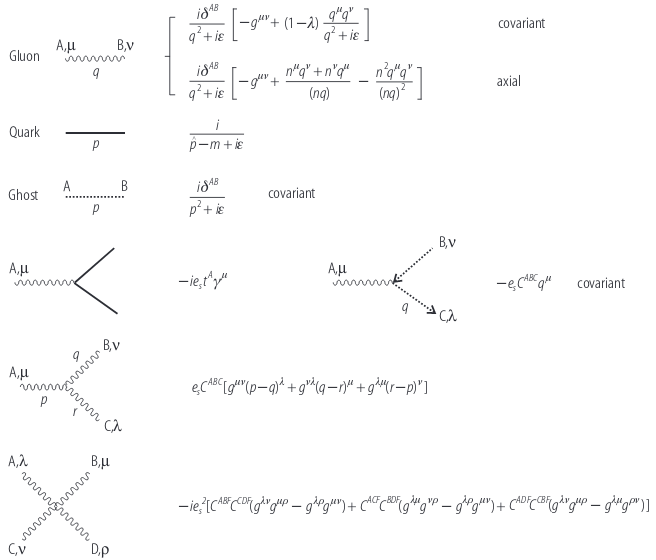
\includegraphics{qcd_feynman.png}
  \caption{The propagators and vertices in QCD along with the corresponding Feynman rules for the amplitude factors \cite{Altarelli:2013tya}. The strong coupling charge is written here as $e_s = \sqrt{4\pi\alpha_s}$, and the gauge parameter is denoted by $\lambda$.}
  \label{fig:qcd_feynman}
\end{figure}

%% The QCD Lagrangian has a symmetry under the gauge transformation defined as... %% we don't really need to get explicit about gauge transformations
The physical interaction vertices of \qcd are a 3-point quark-gluon vertex analogous to the \ac{QED} vertex, a 3-gluon vertex and a 4-gluon vertex (\cref{fig:qcd_feynman}).
A scalar ghost field\footnote{which has a spin of 0 yet anti-commutes like a fermion} also couples to the gluon as is generally necessary in non-abelian gauge theories to prevent over-counting gauge-equivalent states \cite{Faddeev:1967fc}.
The non-abelian nature of \qcd manifests in Feynman diagrams as the gluon self-interaction vertices.
The gluon-gluon interactions make \qcd difficult to apply in theoretical calculations.
In a classical theory, they prevent the principle of superposition from being applied in chromodynamics.
The highly-nontrivial gluon self-interaction is a crucial ingredient in the richness of nuclear physics.


\subsection{Running of the coupling constant} %% maybe doesn't deserve its own section, instead split into UV and IR?

%% https://arxiv.org/pdf/1604.08082.pdf

As is the case in all quantum field theories, the na\"ive calculation of higher-order (in $\alpha_s$) loop diagram integrals contain divergences in the amplitudes.
In many theories, including \qcd \cite{Gross:1973ju}, these infinities can be handled using a process called \emph{renormalization}.
One description of renormalization is the introduction of an energy/momentum cutoff scale.
Physical calculations cannot depend on any such scales, so amplitude calculations must be organized such that any dependence on the renormalization scale cancels in a physical result, which can be done order-by-order in perturbation theory.
This process induces a scale dependence of the coupling constant $\alpha_s$ on the arbitrary renormalization scale $\mu$.
If the value of $\alpha_s$ is known at a particular $\mu = \mu_0$, its dependence on the scale can be determined by calculating the beta function
\begin{equation}
  \beta(\alpha_s) \equiv  \frac{\partial \alpha_s}{\partial \ln \mu^2}
\end{equation}
which to one loop is given by \cite{Gross:1973id}
\begin{equation}
  \beta(\alpha_s) = -b_0 \alpha_s^2 + \bigo{\alpha_s^3}
\end{equation}
where
\[
%% \beta_1 = \frac{11 N_c - 2 N_f}{3}
b_0 = \frac{11 N_c - 2 N_f}{12\pi}
\]
for $N_c$ colors and $N_f$ relevant quark flavors at the scale of the process.
The \ac{LO} solution is
\begin{equation}
  \alpha_s(\mu^2) = \frac{1}{b_0 \ln\left(\mu^2 / \lqcd^2\right)}
  \label{eq:running_as}
\end{equation}
where \lqcd is defined by a given value for $\alpha_s$ at a scale $\mu_0$
\[
\lqcd = \mu_0 \exp \left( -\frac{1}{2 b_0 \alpha_s(\mu_0^2)} \right) \; .
\]
The above expression for \lqcd changes depending on the order of the perturbative expansion and the renormalization scheme, but the physical meaning of \lqcd is still apparent.
It is the energy scale below which the strong coupling diverges, showing an explicit breakdown of perturbation theory.
It is noteworthy that \qcd predicts the emergence of such a scale, even in the conformal\footnote{i.e. a scale-invariant lagrangian with massless quarks} theory.
Practically the \qcd scale is often quoted around a value of %% at the 5-quark level, where \mu ~ m_Z
\[
\lqcd \approx 200 \MeV \;,
\]
but the precise value can differ by a factor of 2 or more depending on arbitrary choices such as scheme, order, and gauge.

A convenient choice for the renormalization scale $\mu$ in \cref{eq:running_as} is to set $\mu^2 = Q^2$ for a physical process with momentum transfer $Q$.
This choice introduces some theoretical and computational wrinkles but gives a simple and direct relationship to experimental data.
Experimental values of the strong coupling constant are typically reported at the mass of the $Z$ boson, with a current world average value of
\[
\alpha_s(m_Z^2) = 0.1181 \pm 0.0011
\]
where $m_Z = 91.187 \GeV$.
The running of the coupling is demonstrated by the summary of experimental measurements in \cref{fig:running_coupling}.

\begin{figure}[t]
  %% page 155 of particle review
  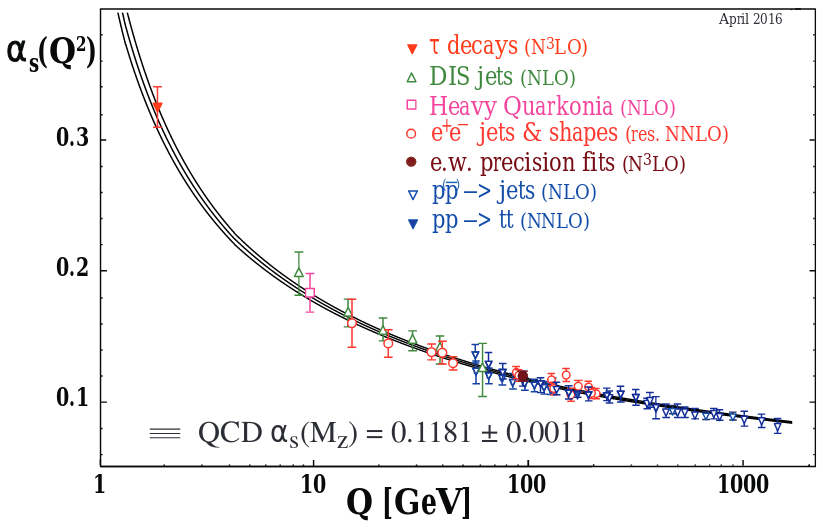
\includegraphics{running_as.png}
  \caption{Measurements of the strong coupling constant $\alpha_s$ as a function of the energy scale $Q$ \cite{Tanabashi:2018oca}.}
  \label{fig:running_coupling}
\end{figure}

\subsection{Asymptotic freedom}

The strong coupling constant decreases with rising energy as shown in \cref{eq:running_as} and \cref{fig:running_coupling}.
This phenomenon is known as \emph{asymptotic freedom} and is necessary to explain Bjorken scaling since without this feature the interaction between quarks bound in a hadron could not be approximately ignored in a \ac{DIS} process.
It requires $b_0 > 0$, which for $N_c = 3$ \qcd is true so long as there is no scale at which additional quark fields become relevant such that $N_f > 16$.
Physically this is understood as arising from the fact that the contributions to $\alpha_s$ from gluon loops dominate over those from quark loops \cite{Wilczek:2005az}.

Asymptotic freedom is not present in abelian gauge theories like \ac{QED}, where the screening of a bare electric charge causes the effective charge to decrease at large distances, or equivalently the effective electric charge increases at higher energy.
In \qcd the color field reinforces itself to induce an even stronger field so the effective field strength does not decrease with increasing separation.

The phenomenology of jets relies heavily on asymptotic freedom.
In high energy hadronic and nuclear collisions, partons from each participant nucleon scatter with large momentum transfer.
Because the effective $\alpha_s$ is small, the product quarks and gluons are ejected with large transverse momentum and are not strongly coupled to other partons in the collision.
The stronger coupling at low $Q^2$ also means that the \qcd radiation is emitted at small relative momentum from the hard parton.
Thus the decay products of these high-energy partons are produced in a \emph{parton shower} and generate clumps of final-state particles known as jets.

\subsection{Color confinement}

In order to be trusted as a fundamental theory of nuclear interactions, \qcd must provide an understanding of the lack of experimental observation of free quarks or gluons.
Indeed the infrared divergence of $\alpha_s(Q^2)$ suggests that there is some nontrivial behavior as the separation between two colored particles is increased.
Predictions from \qcd in this region cannot be investigated using perturbation theory since the rapidly rising coupling constant precludes the convergence of any diagram expansion.
The numerical approach of \emph{lattice gauge theory} \cite{Aoki:2016frl} is successful at reproducing a number of experimental measurements such as the light hadron mass spectrum \cite{Durr:2008zz}.
Lattice gauge theory introduces a discrete grid spacing $a$ along both spatial and temporal dimensions, which acts as a regularization parameter.
An extrapolation to a vanishing grid spacing $a \rightarrow 0$ is performed in order to recover the continuous theory of \qcd.

\begin{figure}[t]
  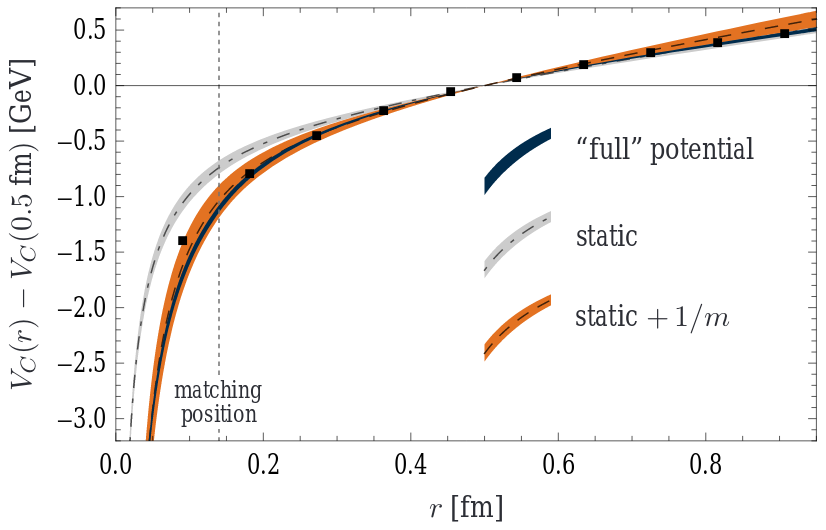
\includegraphics{ccbar_potential.png}
  \caption{Charmonium ($c\bar{c}$) potential from a combination of perturbative QCD (small $r$) and lattice QCD (large $r$) \cite{Laschka:2011zr}.}
  \label{fig:charmonium_potential}
\end{figure}

The heavy quark-antiquark potential can be computed with \ac{pQCD} at small separations and on the lattice for large separations, as shown in \cref{fig:charmonium_potential}.
The charmonium lattice \qcd potential with three light quarks and charm-quark mass effects is well-described to the 4-loop level by the parameterization \cite{Laschka:2011zr}
\begin{equation}
V_{c\bar{c}}(r) = - \frac{A}{r} + \sigma r
\end{equation}
with $A = 160 \pm 4 \MeV\,\fm$ and $\sigma = 790 \pm 30 \MeV/\fm$ (\cref{fig:charmonium_potential}).
The first term has the same form as an attractive Coulomb potential, albeit with a coupling constant about 2 orders of magnitude larger than the \ac{EM} coupling\footnote{where $\alpha_\textrm{EM} \hbar c \approx 1.44 \MeV\,\fm$}.
The latter term resembles the potential from the force by a string of constant tension $\sigma$.
This invokes a description of the force between the two quarks as color ``flux tubes'' of constant energy per length.
The ``string'' term $\sigma$ increases without bound at large separations so a quark-antiquark pair cannot be separated with a finite amount of energy.
At some point it becomes more energetically favorable to produce a quark-antiquark pair out of the vacuum than to maintain a long flux tube (\cref{fig:qqbar_flux}).
This property is responsible for the phenomenon of \emph{confinement}, which is the absence in nature of bare color charges.

\begin{figure}[t]
  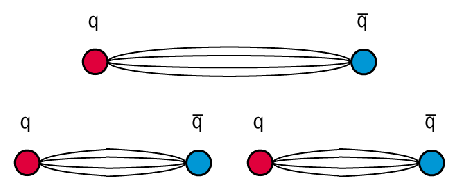
\includegraphics{qqbar_flux.png}
  \caption{The color flux tube between a quark-antiquark pair and the breaking of the flux tube into a new $q\bar{q}$ pair from the vacuum.}
  \label{fig:qqbar_flux}
\end{figure}

%% \todo{possibly add detail on lattice gauge theory}

\section{QCD at high temperatures}

Given the observed properties of asymptotic freedom and color confinement, a natural question to ask is whether nuclear matter has a phase transition at large density and/or temperature.
In a system with a low number of quarks, the color connection keeps each bound tightly to others.
At high densities, however, individual flux tubes are not discernible, and individual color charges are easily balanced by nearby color sources.
Such a state could exhibit deconfinement, with color charge free to move as electric charge does in a conventional plasma.
This \qgp is expected to have different properties than hadronic matter.

\begin{figure}[t]
  %% https://homepages.uni-regensburg.de/~sow28704/ftd_lqcd_ss2012/ftd_lqcd_ss2012.html
  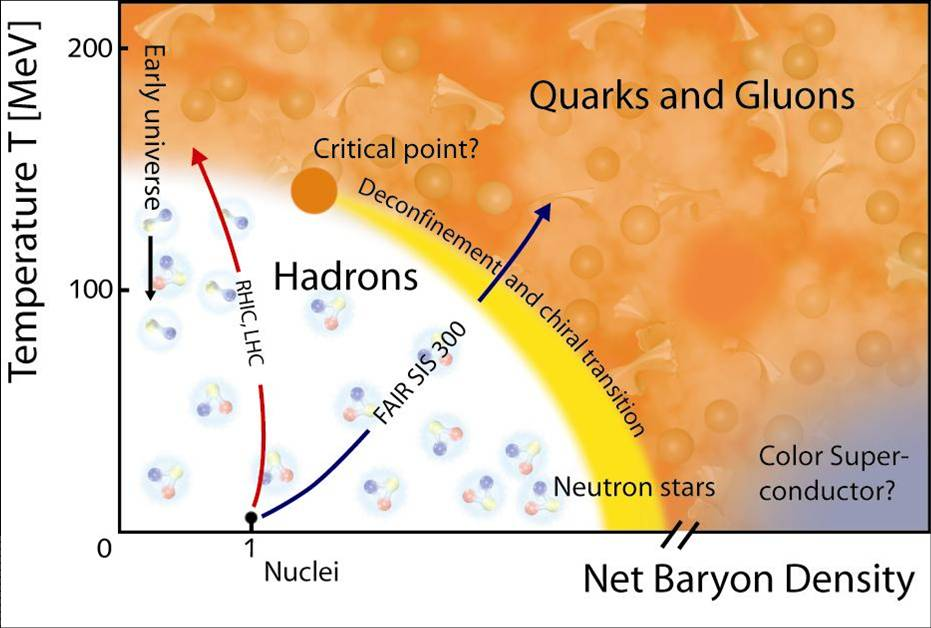
\includegraphics{qcd_phase.jpg}
  \caption{A conjectured phase diagram for QCD matter. The transition from hadronic matter to QGP at low baryon density is a smooth crossover. A critical point is hypothesized but not established.}
  \label{fig:qcd_phase}
\end{figure}

Dimensional analysis suggests that the critical temperature $T_c$ (at zero chemical potential) should be close to the only possibly relevant scale
\[
T_c \sim \lqcd \sim 10^{12}~\mathrm{K}\; .
\]
\cref{fig:qcd_phase} shows a conjectured phase diagram for \qcd matter.
The transition between hadronic matter and the QGP is a smooth crossover at low baryon density \cite{Aoki:2006we}.
Above some critical baryon density the transition is hypothesized to be first-order based on a number of model approaches, but this has not been established.
The existence of such a critical point, along with its temperature and density in the phase diagram, is an objective of experimental measurements particularly at \ac{RHIC}.

\subsection{Ultrarelativistic thermodynamics}
For particles of negligible mass the probability of having energy $E$ is calculated by integrating over the constrained phase volume \( \frac{d^3 x \, d^3 p}{(2\pi)^3} \delta\left( E - |\mathbf{p}|\right)\) times the density of states.
With the statistical factor $\eta=\pm1$ for bosons/fermions and $\eta=0$ for non-identical particles, this gives a probability per unit volume of
\begin{equation}
\frac{g E^2}{2\pi^2} \frac{1}{e^{E/T} - \eta}
\end{equation}
where $g$ is a degeneracy factor e.g. for multiple spin values.
%% \begin{align}
%%   \varepsilon_\textrm{NI} =& g\frac{3T^4}{\pi^2} \\
%%   n_\textrm{NI} =& g\frac{T^3}{\pi^2}
%% \end{align}
This yields expressions for the energy and number density of bosons
\begin{align}
  \varepsilon_\textrm{BE} =& g\frac{\pi^2 T^4}{30} \\
  n_\textrm{BE} =& g\frac{\zeta(3) T^3}{\pi^2}
\end{align}
and fermions
\begin{align}
  \varepsilon_\textrm{FD} =& g\frac{7 \pi^2 T^4}{240} = \frac{7}{8} \varepsilon_\textrm{BE} \\
  n_\textrm{FD} =& g\frac{3 \zeta(3) T^3}{4 \pi^2} = \frac{3}{4} n_\textrm{BE} \; .
\end{align}
Relative to the energy and number density for non-identical particles, quantum statistical effects increase the density for bosons and decrease it for fermions.

For a non-interacting mixture the total energy density is
\begin{equation}
\varepsilon = \left( g_\textrm{BE} + \frac{7}{8} g_\textrm{FD} \right) \frac{\pi^2 T^4}{30}
\end{equation}
where the $g$ terms are the total degeneracy factors for relevant particle species.
For instance, at low temperatures where a system is hadron gas the degrees of freedom are the pions with 3 isospin possibilities, so $g_\textrm{BE} = 3$ and $g_\textrm{FD} = 0$.
In \qcd the energy density becomes\footnote{Gluons have $3^2 - 1 = 8$ possible colors and 2 possible spins, while each flavor of quark has 3 possible colors and 4 spinor components.}
\begin{equation}
  \label{eq:qcd_energy}
\varepsilon = \left( 32 + 21 N_f \right) \frac{\pi^2 T^4}{60}
\end{equation}
for $N_f$ active quark flavors at the temperature scale.
At a phase transition where the active thermodynamic degrees of freedom become quarks and gluons from pions the ratio $\varepsilon/T^4$ would be expected to increase by an order of magnitude.

\subsection{Thermal quantum field theory}
The probability of a thermal system to be in state $\psi$ is proportional to $e^{-\beta H(\psi)}$ where $\beta = 1/T$ is the coldness and $H$ is the Hamiltonian of the configuration.
This is generally expressed in terms of the partition function
\begin{equation}
  \label{eq:z_classical}
Z(\beta) = \mathrm{tr} \left( e^{-\beta H} \right)
\end{equation}
so that the thermodynamic expectation value of an operator $\mathcal{O}$ is given by
\begin{equation}
\langle \mathcal{O} \rangle = \frac{1}{Z} \mathrm{tr} \left( \mathcal{O} e^{-\beta H} \right) \;.
\end{equation}
In \ac{QFT} the partition function is represented by the path integral
\begin{equation}
  \label{eq:z_qft}
  Z = \int \mathcal{D}[\psi] \, e^{i\int d^4 x \, \Lagr(\psi)}
\end{equation}
from which amplitudes can be calculated through functional derivatives of $Z$ with source terms $J \cdot \psi$ in the Lagrangian density.
At the same time, by analogy with \cref{eq:z_classical} the thermal partition function must look something like
\begin{equation}
  \label{eq:z_analogy}
Z \sim \int \mathcal{D}[\psi] \, e^{-\beta \int d^3 \mathbf{x} \, \mathcal{H}(\psi)}
\end{equation}
in terms of the Hamiltonian density $\mathcal{H}$.
The Lagrangian can be related to the Hamiltonian by a Wick rotation $t \rightarrow -i\tau$ which transforms $\mathcal{L} \rightarrow - \mathcal{H}$.
With the transformation of the temporal integral in the exponent $i \int dt$ into a periodic domain $\int_0^\beta d\tau$ this analogy can be made precise.
The fields are periodic such that \(\psi(\beta,\mathbf{x}) = \pm \psi(0,\mathbf{x})\) where the sign is determined by whether the field is a boson or fermion.
This periodicity leads to discretization of the allowed energies where $E_n = 2n\pi T$ for bosons and $E_n = (2n+1)\pi T$ for fermions.

With this formalism the full power of perturbation theory can be applied to calculate a number of observables \cite{Gross:1980br}.
The real-time tree-level propagators pick up absorptive terms proportional to \(2\pi \delta(p^2 - m^2) \frac{1}{e^{|p^0|/T} \mp 1} \) for bosons/fermions.
For instance, computation of the free energy $ -T \log Z$ leads to a corresponding \ac{LO} correction to \cref{eq:qcd_energy}.
\begin{equation}
  \label{eq:qcd_energy_lo}
\frac{\varepsilon}{T^4} = \left( \frac{4\pi}{15} - \alpha_s \right)2\pi + \left(\frac{7\pi}{10} - \frac{5}{3}\alpha_s \right)\frac{\pi N_f}{2}
\end{equation}


\subsection{Equation of state from lattice calculations}
\label{subsec:lattice}

\begin{figure}[t]
  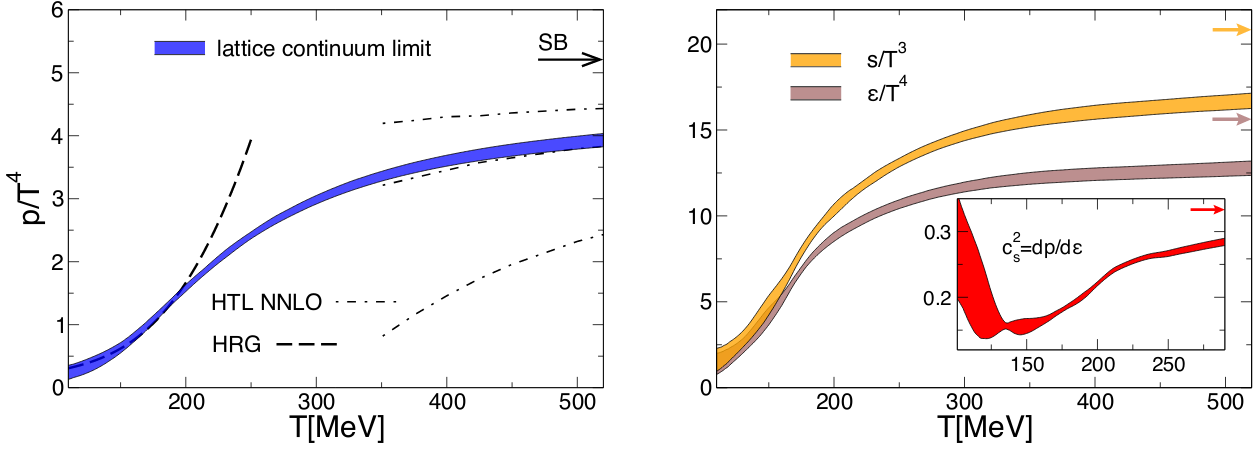
\includegraphics[width=\linewidth]{lattice_eos.png}
  \caption{The trace anomaly for several values of lattice spacing $N_\tau = 1/aT$ and the continuum extrapolation (left) and thermodynamic quantities in the continuum limit (right), both shown as a function of temperature \cite{Bazavov:2014pvz}. The solid lines show the predictions from the hadron resonance gas model and the Stefan-Boltzmann limit for 3 quark flavors at $19\pi^2/12$ is shown by the straight dashed line.}
  \label{fig:lattice_eos}
\end{figure}

%% the latter HotQCD ref is slightly more recent and has many good plots including static potential (no 1/m corrections?)
Thermodynamic quantities can be computed in lattice \qcd at small chemical potential \cite{Borsanyi:2013bia,Bazavov:2014pvz}.
The results are clearly distinct from the \ac{HRG} model \cite{Huovinen:2009yb}, indicating that deconfinement is a fundamental property of the transition.
The trace anomaly $T_\mu^\mu = \varepsilon - 3 p$, where $\varepsilon$ is the energy density and $p$ is the pressure, is computed in lattice calculations as a function of temperature.
It vanishes in a conformal theory, so the appearance of a significant trace anomaly with a peak around $200 \MeV$ suggests the emergence of a scale dependence.
The pressure is related to the derivative of the trace anomaly up to factors of the temperature.
From there, the remaining combinations of thermodynamic quantities such as $\varepsilon(T)$ and the entropy density $s = \frac{\varepsilon + p}{T}$ are computed, determining the \ac{EoS}.

Recent lattice \qcd results are shown in \cref{fig:lattice_eos}.
The large step in the ratios $\varepsilon/T^4$ and $s/T^3$ around the critical temperature suggests a phase transition indicated by the increase in the effective number of degrees of freedom in \qcd matter.
A smooth crossover is observed with a critical temperature of \( T_c = 170 \pm 4 \MeV \) \cite{Aoki:2009sc}, which is indeed close to \lqcd as predicted by dimensional analysis.
Above the critical temperature, clear deviations are shown from the predictions of the \ac{HRG} model.
The Stefan-Boltzmann limit does not appear to be reached, which appears to be consistent with \cref{eq:qcd_energy_lo} which says that perturbative corrections to the energy are negative.


\subsection{Heavy ion collisions}

Heavy ions, like gold-197 and lead-208, have hundreds of nucleons packed into a spherical volume of radius $\sqrt[3]{A} \approx 6$ times that of a proton.
This also corresponds to an average transverse areal density of the same factor of 6 times larger than that of a proton.
In a head-on \AuAu or \PbPb collision, roughly 200 times the matter interacts in a transverse area about 35 times larger than a \pp collisions of the same $\sqrt{s_\mathrm{NN}}$.
The high densities and temperatures reached in these collisions allow for the potential to produce deconfined \qgp matter.
%% Hydrodynamic modeling suggests a formation time on the order of 1 fm/c, so na\"ively the ultra-relativistic initial products of nuclear collisions have the potential to reach thermalization in \AA collisions.

\begin{figure}[t]
  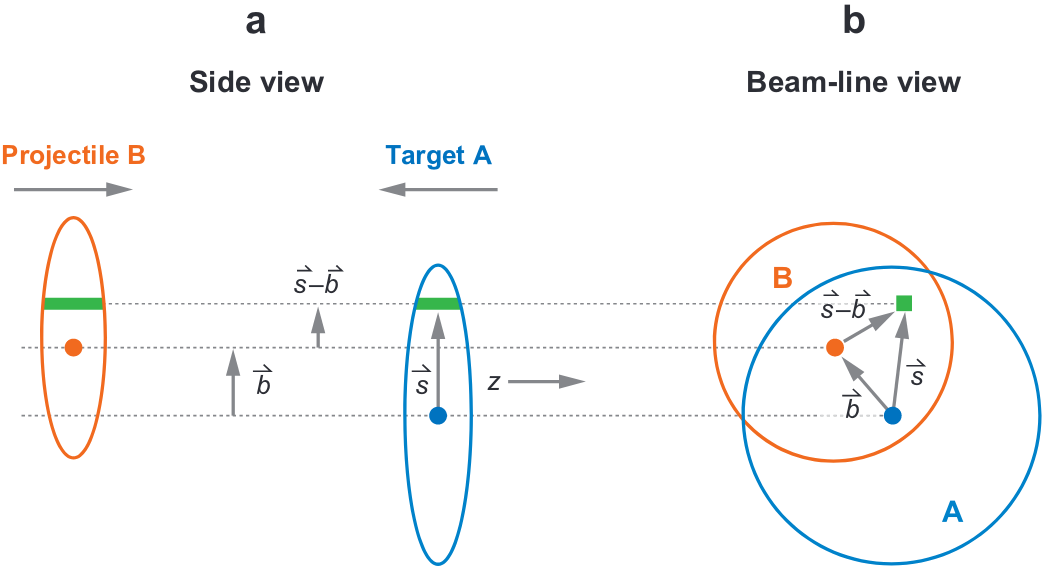
\includegraphics{hi_collision_geo.png}
  \caption{Diagram of the Glauber model nucleus-nucleus geometry with transverse (a) and longitudinal (b) perspectives \cite{Miller:2007ri}.}
  \label{fig:hi_collision_geo}
\end{figure}

The size and shape of the energy density deposited in a heavy ion collision varies greatly depending on the impact parameter $b$, as illustrated in \cref{fig:hi_collision_geo}.
The Glauber model is used to describe the average energy density in nuclear collisions as a function of impact parameter \cite{Miller:2007ri}.
In the optical limit of smooth density, the nuclear density $\rho$ is parameterized by the Woods-Saxon distribution
\begin{equation}
\rho(r) = \frac{\rho_0}{1 + \exp\left( \frac{r-R}{a} \right)} \, ,
\end{equation}
where $R$ and $a$ are the radius and skin depth of the nucleus, respectively.
The normalization constant \[\rho_0 = \frac{3A}{4 \pi R^3} \left[1 + \frac{\pi^2 a^2}{R^2}  + \bigo{e^{-R/a}}\right]^{-1}\] is set to fix the integral to the total number of nucleons\footnote{The exact expression in terms of the trilogarithm function is \( \rho_0 = \frac{A}{-8\pi a^3 \mathrm{Li}_3\left( -e^{R/a} \right)} \).}.
The radial density distribution for lead-208 is shown in \cref{fig:woods_saxon}, with $R = 6.62 \pm 0.06~\fm$ and $a = 0.55 \pm 0.01~\fm$.

\begin{figure}[t]
  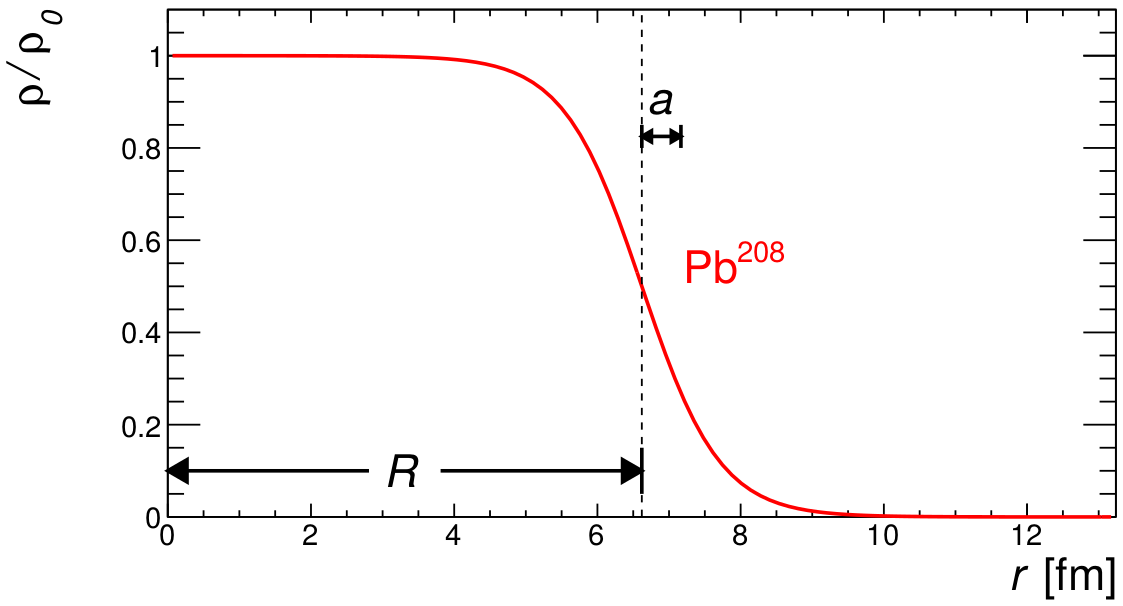
\includegraphics{woods_saxon_pb208.png}
  \caption{The density as a function of radius following the Woods-Saxon distribution for the ${}^{208}\mathrm{Pb}$ nucleus.}
  \label{fig:woods_saxon}
\end{figure}

The transverse density of a nucleus with mass number $A$ at a transverse position $\mathbf{s}$ relative to its center is given by the projection of the spherical density along a longitudinal axis.
\begin{equation}
T_A(\mathbf{s}) = \int dz \, \rho_A\left( \sqrt{s^2 + z^2} \right)
\end{equation}
For two nuclei with mass numbers $A$ and $B$ colliding with impact parameter $\mathbf{b}$, the thickness function is
\begin{equation}
T_{AB}(\mathbf{b}) = \int d^2 b \, T_A(\mathbf{s}) T_B(\mathbf{s} - \mathbf{b}) \;,
\end{equation}
which has units of inverse area.
The expected number of nucleon-nucleon collisions \Ncoll is obtained by multiplying the thickness function by the inelastic nucleon-nucleon cross-section\footnote{More rigorously, the probability distribution of \Ncoll for a given impact parameter $b$ is the binomial distribution $B(n,p)$ with $n = AB$ and $p = \frac{T_{AB}(b) \sigma^{NN}_\mathrm{inel}}{AB}$. }
\begin{equation}
  \langle\Ncoll(b)\rangle = T_{AB}(b) \sigma^{NN}_\mathrm{inel} \;.
\end{equation}
%% The inelastic nucleus-nucleus cross-section is
%% \begin{equation}
%% \frac{d^2 \sigma^{AB}_\mathrm{inel}}{db^2} = 1 - \left[ 1 - \frac{T_{AB}(b) \sigma^{NN}_\mathrm{inel}}{AB} \right]^{AB} \;.
%% \end{equation}
The number of nucleons in both target and projectile that interact is called the number of participating nucleons, \Npart, or the number of wounded nucleons.
\begin{equation}
  \begin{split}
  \langle \Npart(b) \rangle = &\int d^2 s \, T_A(\mathbf{s})\left\{ 1 - \left[ 1 - \frac{T_B (\mathbf{s} - \mathbf{b}) \sigma^{NN}_\mathrm{inel}}{B} \right]^B \right\} + \\
  &\int d^2 s \, T_B(\mathbf{s}-\mathbf{b})\left\{ 1 - \left[ 1 - \frac{T_A (\mathbf{s}) \sigma^{NN}_\mathrm{inel}}{A} \right]^A \right\}
  \end{split}
\end{equation}

The optical approximation taken here is not able to account for fluctuations in nucleon positions within the nuclei.
To remedy this, a \mc approach can be taken which randomizes the impact parameter according to $P(b) \propto 2\pi b$ and the positions of the nucleons within each nucleus according to the Woods-Saxon distribution.
One method is to tag a nucleon as wounded if its distance in the transverse plane is within $\sqrt{\sigma^{NN}_\mathrm{inel}/\pi}$ of any nucleon in the other nucleus.
The expectation values of \Ncoll and \Npart can be calculated as a function of $b$ by repeated simulations. 
The Glauber \mc model predicts some shadowing of the total nucleus-nucleus cross-section relative to the optical approach, but differences in the expected \Ncoll and \Npart are negligible \cite{Miller:2007ri}. %% todo: show figure 5 from this reference here? probably not

In experiments the impact parameter cannot be measured directly so a proxy must be used.
This is typically the charged-particle multiplicity or the total energy deposited at large $|\eta|$.
Because there is a probabilistic component to the particle production at a given $b$, results are often reported in intervals of event activity, either in percentile or the corresponding expected \Npart.

\subsection{Proton-nucleus collisions}
The initial motivation for studying proton-nucleus collisions is to understand \ac{CNM} effects.
Measurements from \AA collisions are often normalized by the same quantities in \pp collisions up to factors of \Npart.
Heavy ion collisions are not completely equivalent to a sum of several \pp collisions, due in part to the presence of additional spectator nucleons.
Proton-nucleus collisions can be used to control for these effects.
The physics of \pA collisions has also turned out to be surprisingly interesting in its own right.

In \pA collisions the expected number of collisions is given in terms of the single-nucleon thickness function
\begin{equation}
  \langle \Ncoll(b) \rangle = T_A(b) \sigma^{NN}_\mathrm{inel}
\end{equation}
and the number of nucleon participants is simply
\begin{equation}
  \Npart = \Ncoll + 1 \;.
\end{equation}
Because the projectile consists of a single proton, event-by-event fluctuations in its size can impact the \Npart significantly.
In \AA collisions the effect of such fluctuations is washed out because the relative fluctuations in the projectile cross-section are suppressed by a factor of $A^{-1/2}$.
The \ac{GGCF} model provides the framework to describe this effect by parameterizing fluctuations in $\sigma^{NN}_\mathrm{inel}$ with the dimensionless parameter $\omega_\sigma$.
The \Npart distribution is shown in \cref{fig:ggcf_npart} for the Glauber model and two values of the \ac{GGCF} extension.
Fluctuations in $\sigma^{NN}_\mathrm{inel}$ put higher weight into the high-\Npart tail of the distribution.

\begin{figure}[t]
  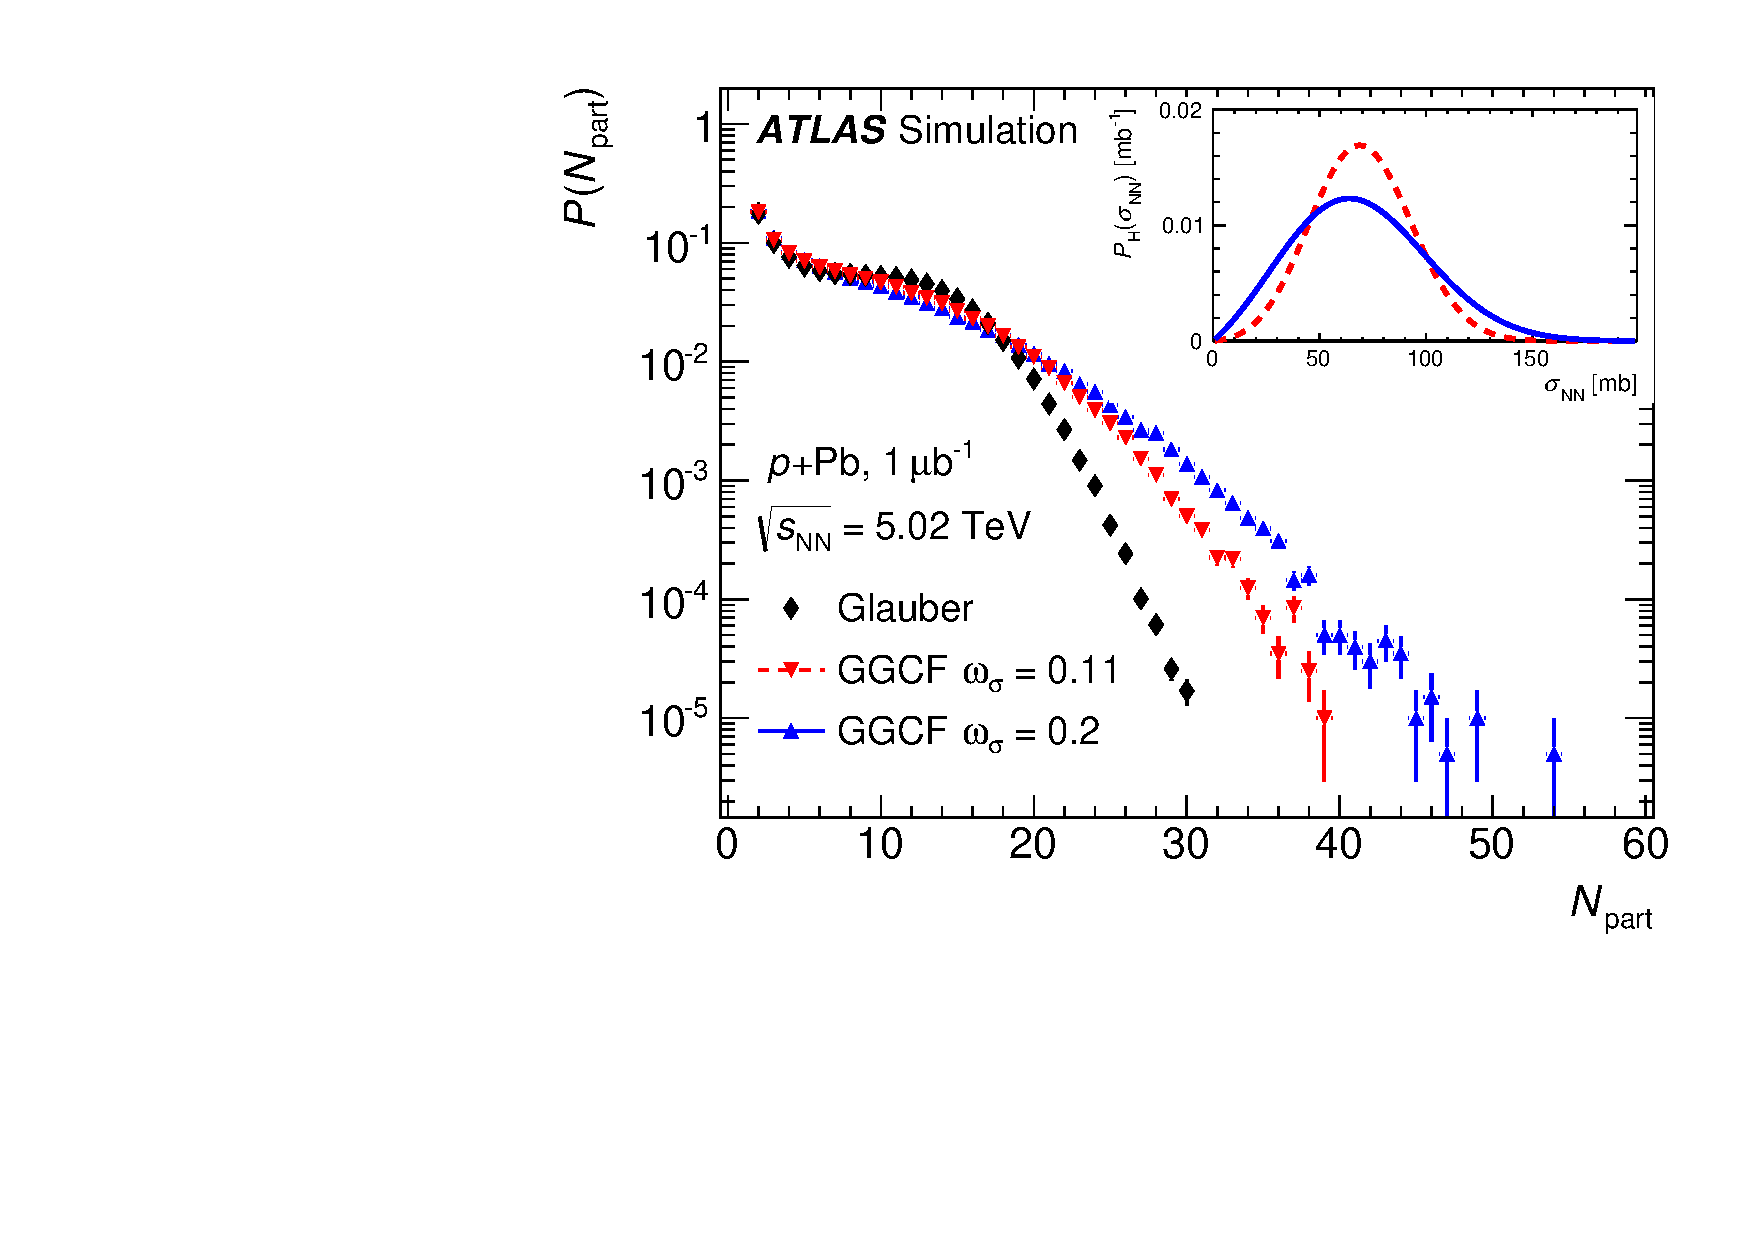
\includegraphics[width=0.49\linewidth]{ggcf_prob_dist.pdf}
  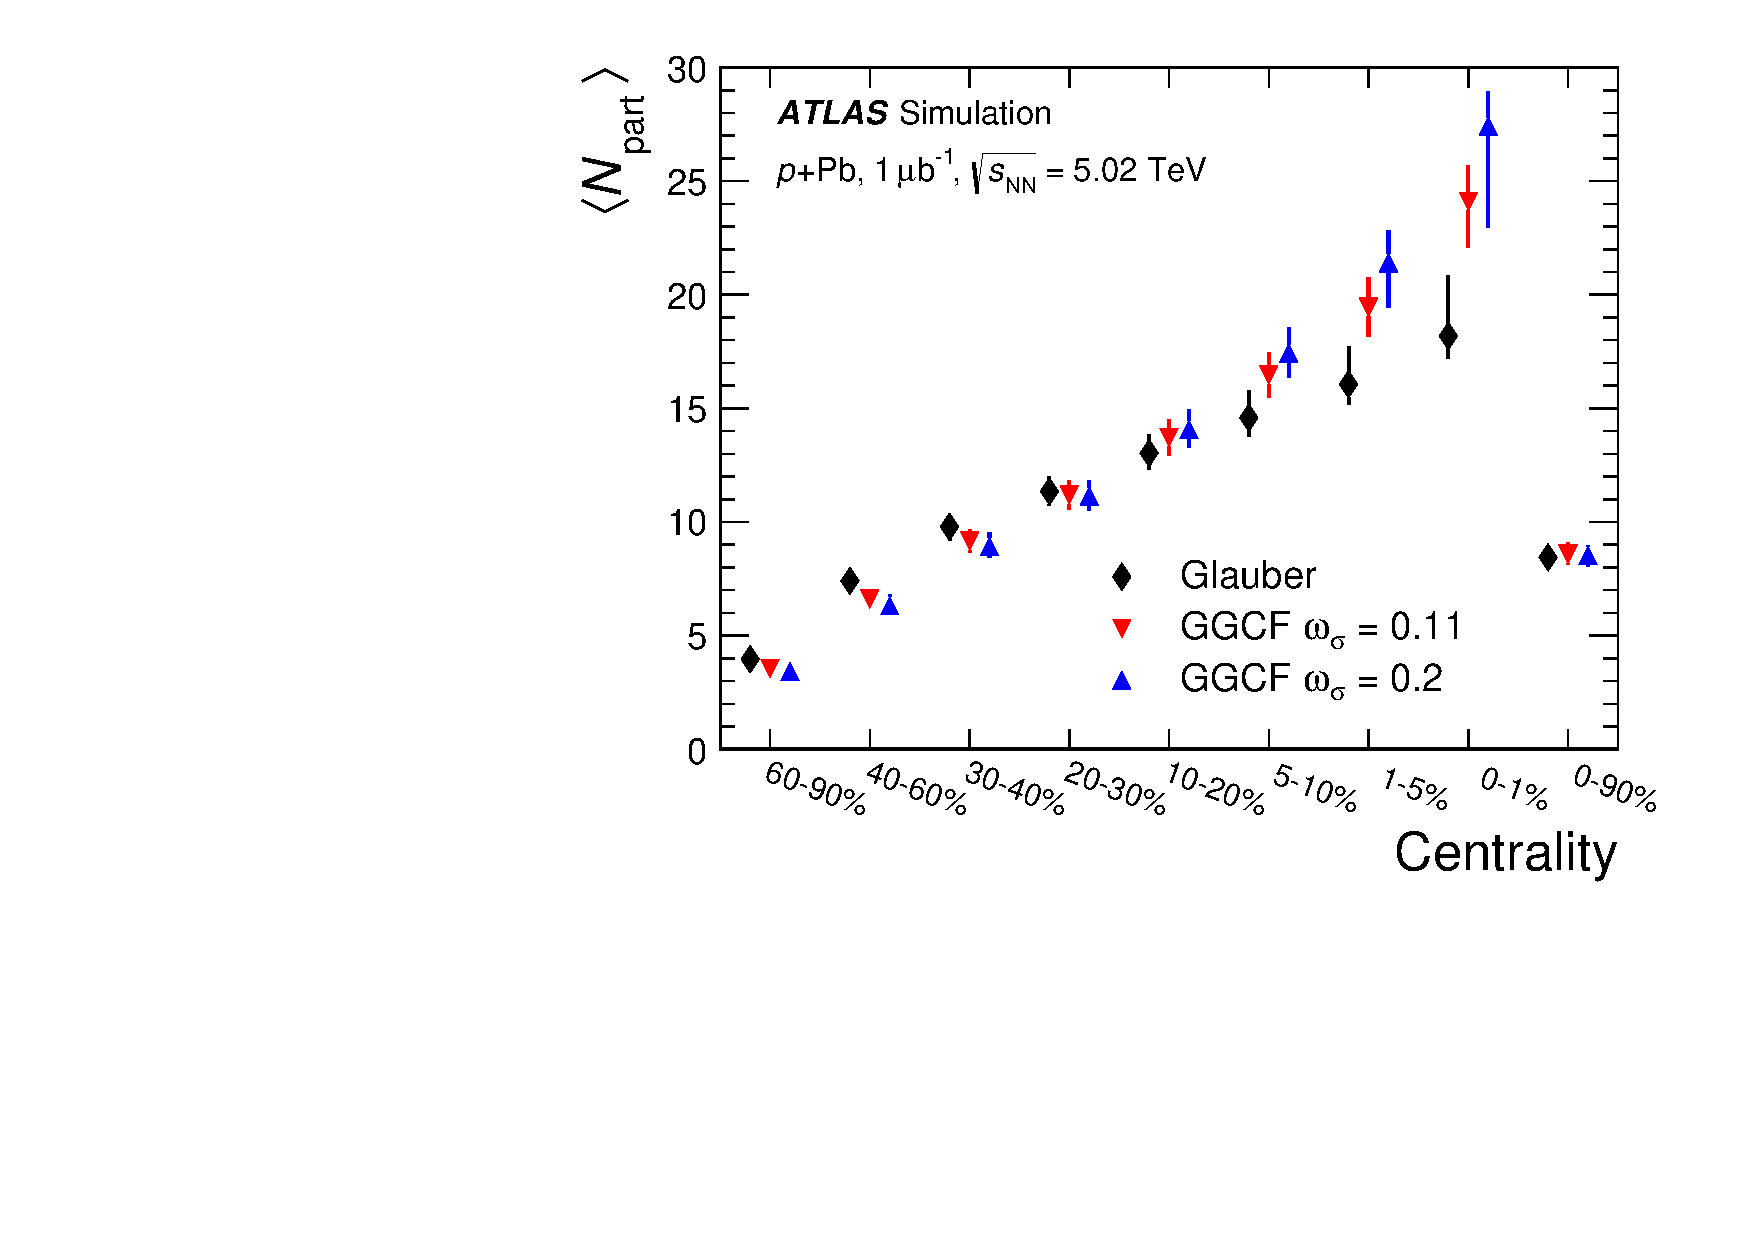
\includegraphics[width=0.49\linewidth]{npart_ggcf.pdf}
  \caption{The \Npart distribution for proton-lead collisions using the Glauber model and the generalized color fluctuation model (left), along with the \avgNpart for the corresponding centrality intervals with each model (right) \cite{HION-2012-15}.}
  \label{fig:ggcf_npart}
\end{figure}

Measurements of charged particle multiplicity and $Z$ boson production suggest that the geometry is best described by $\omega_\sigma > 0$ \cite{HION-2012-15,HION-2013-09}.
The precise value is not well-constrained but a value of $\omega_\sigma = 0.11$ is slightly preferred over the higher value of $0.2$.
Results presented in this thesis will provide additional support for the \ac{GGCF} model with $\omega_\sigma > 0$.


\subsection{Experimental status of the strongly-coupled QGP}

\subsubsection{Hard sector}

\begin{figure}[t]
  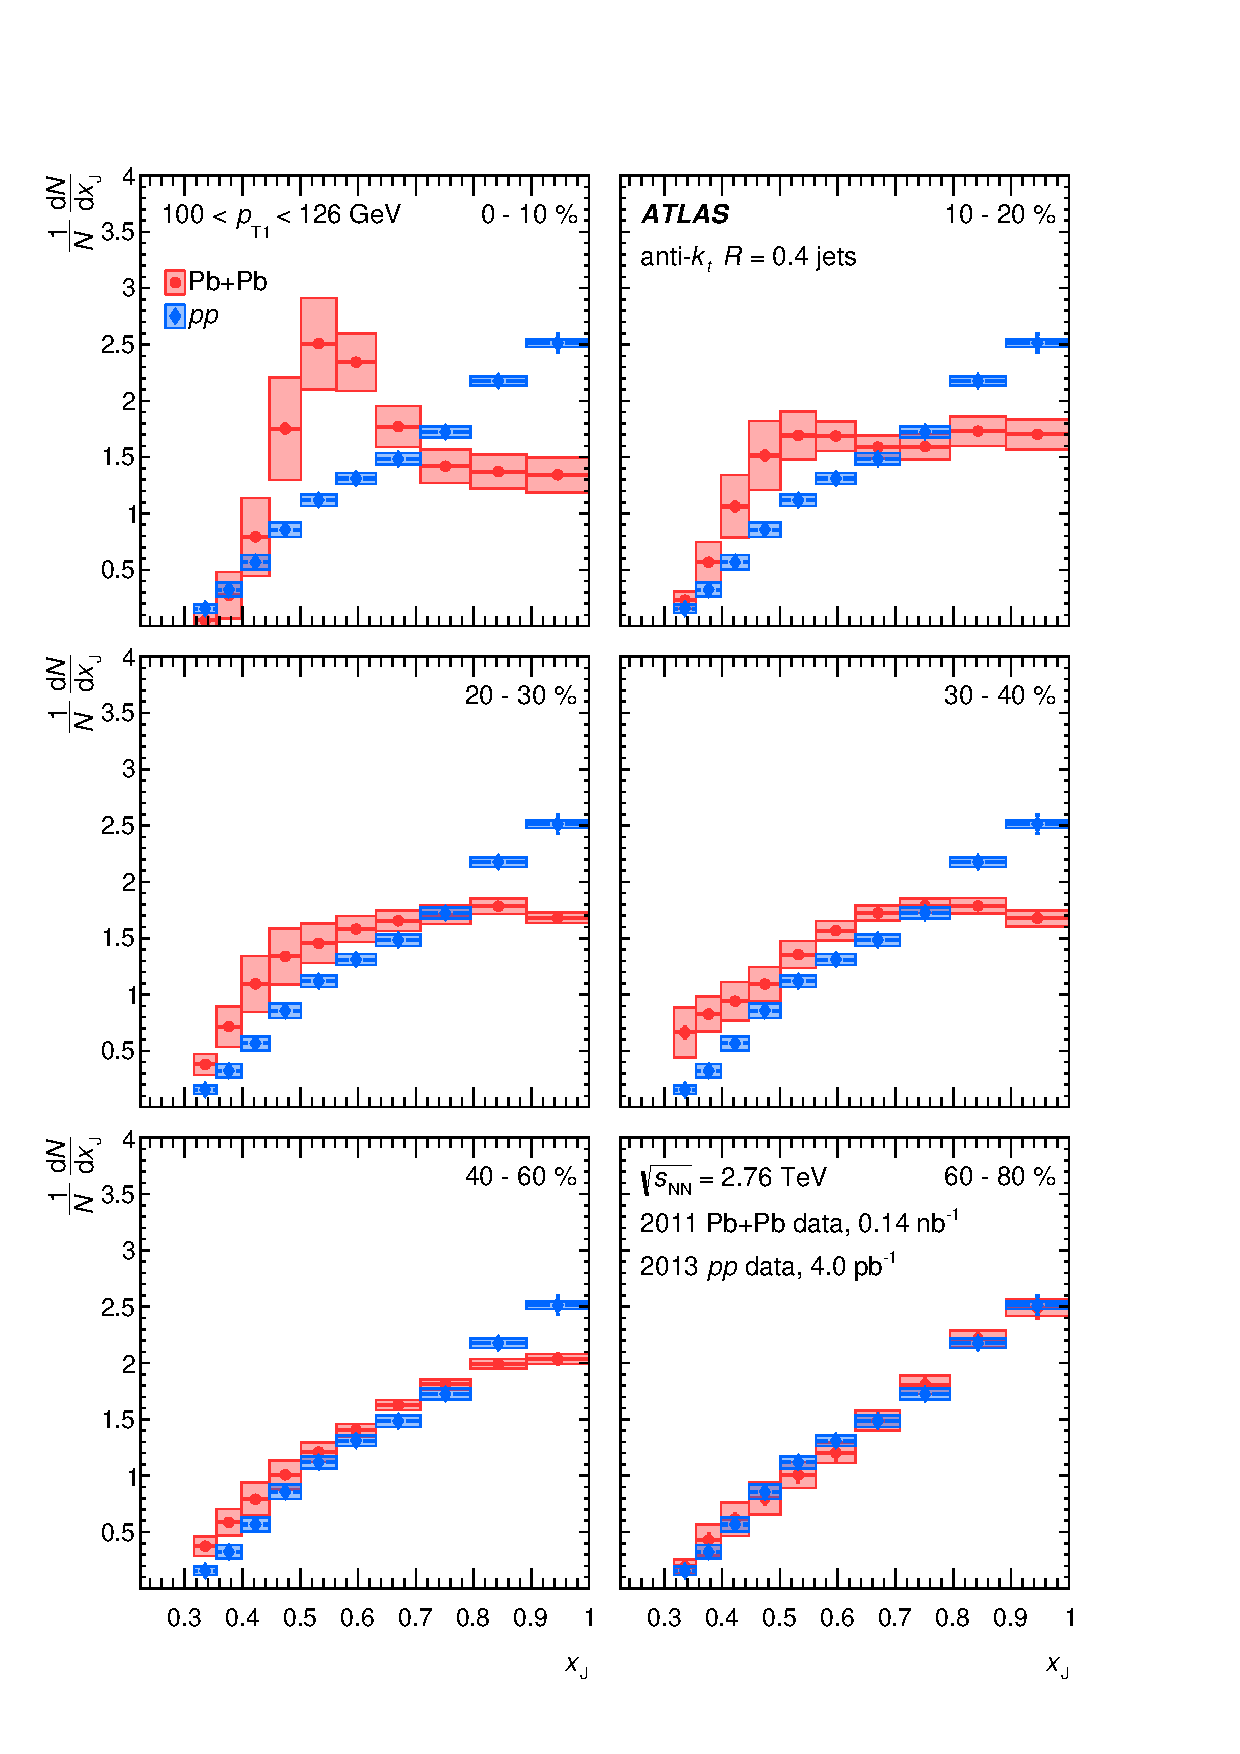
\includegraphics{dijet_asym.pdf}
  \caption{The distribution of the sub-leading jet suppression $x_\textrm{J}$ as a function of centrality in lead-lead collisions \cite{HION-2012-11}. The observable $x_\textrm{J}$ is defined as the ratio of sub-leading to leading jet \pt and is reduced relative to proton-proton collisions. The distributions are unfolded to correct for detector resolution effects.}
  \label{fig:dijet_asym}
\end{figure}

The observation of jet quenching in \PbPb collisions is a signature of the formation of an opaque medium \cite{HION-2012-11}.
The reduction of the ratio of sub-leading jet \pt to leading jet \pt indicates that one of the jets travels a greater apparent distance through a medium.
This effect is drastic in central collisions but not significant in peripheral collisions as shown in \cref{fig:dijet_asym}.
This matter is likely composed of relatively soft particles since if the energy loss was a result only of repeated hard scattering then dijets would be deflected out of a co-linear plane.
Dijet asymmetry has not been observed in \pA collisions, but this does not necessarily rule out the formation of a medium because it could have a formation time comparable to the transverse size of the system.

\begin{figure}[t]
  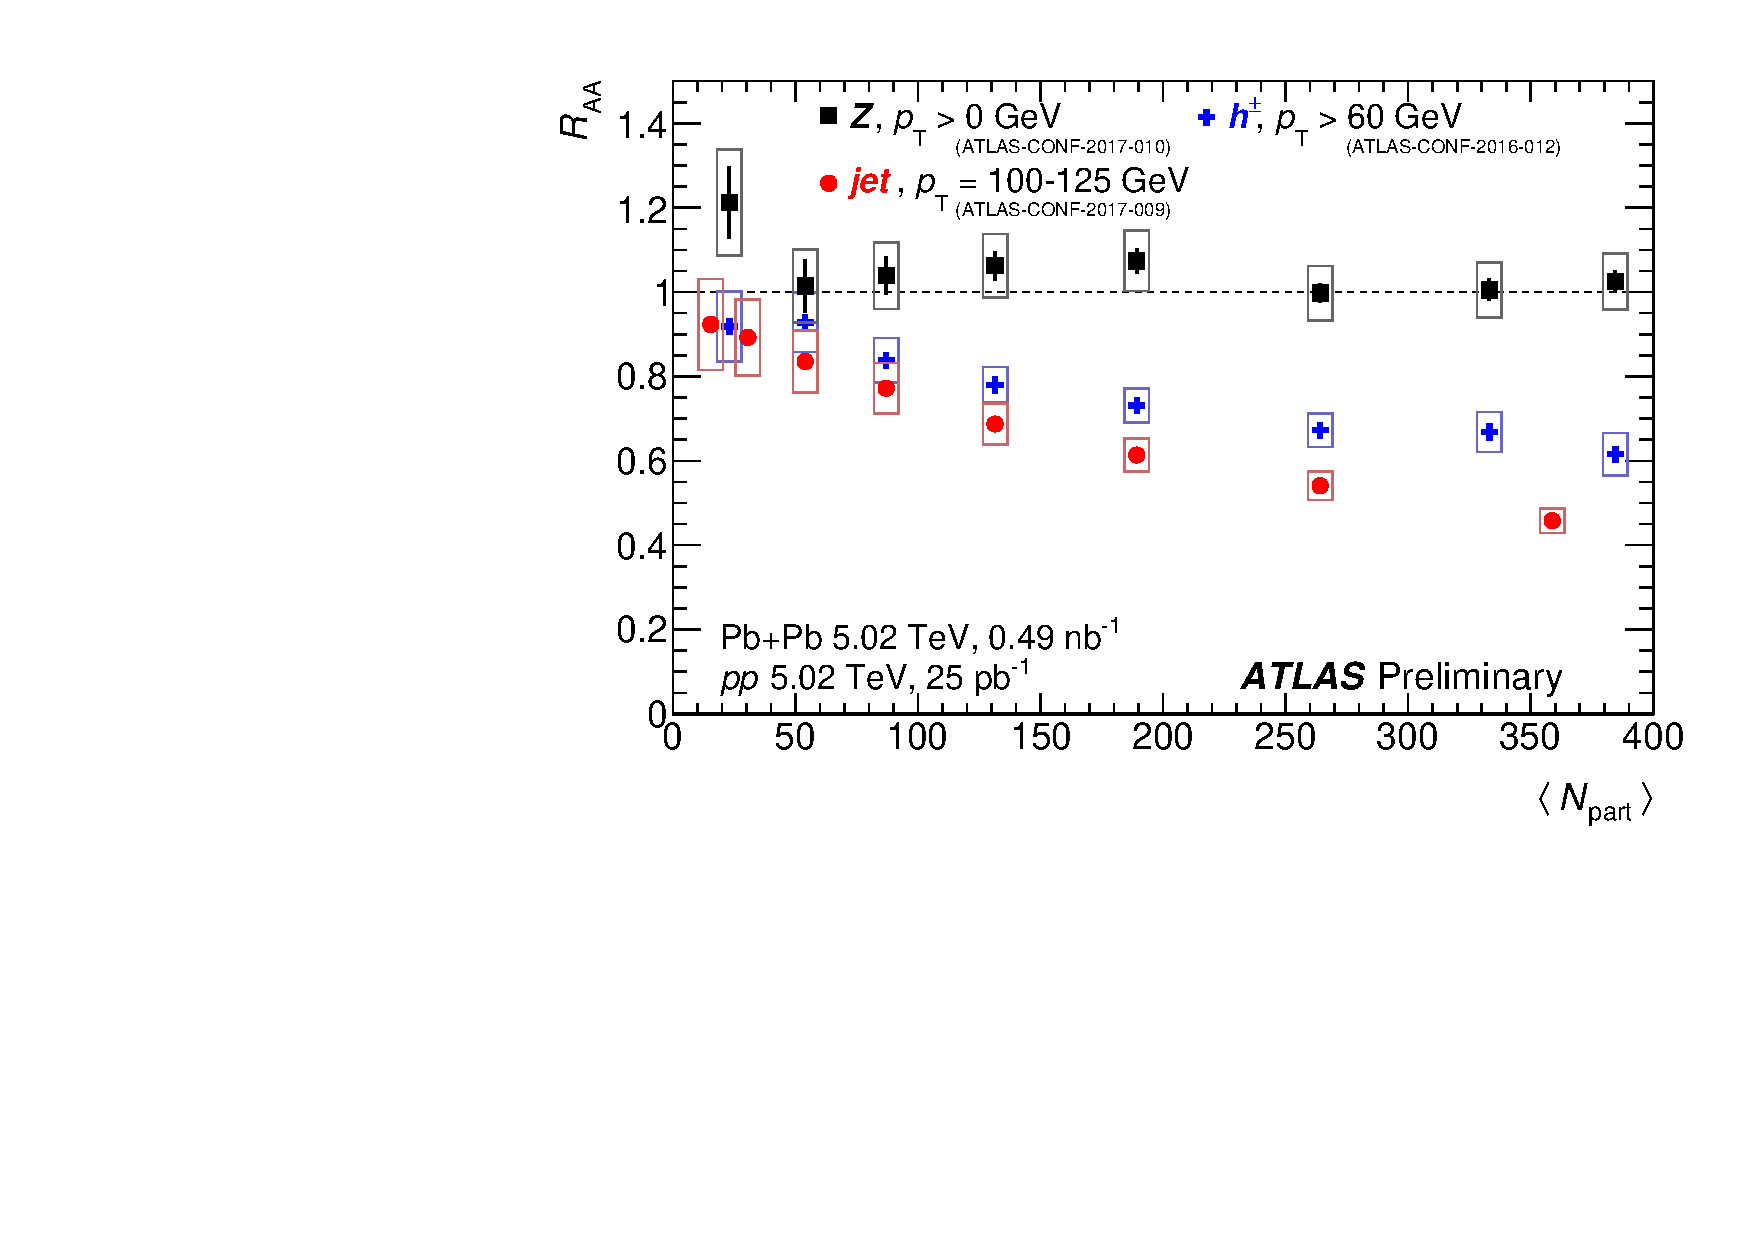
\includegraphics{ATLAS_HION_Summary_Raa_02.pdf}
  \caption{Summary of the nuclear modification factor \RAA for a few relevant production channels in lead-lead collisions. No suppression is observed for the colorless $Z$ bosons, but high-\pt jets and hadrons are suppressed with an increased effect in central collisions.}
  \label{fig:pbpb_raa}
\end{figure}

Jet and particle production in heavy ion collisions is often reported in terms of the nuclear modification factor \RAA of channel $X$.
\begin{equation}
  \RAA = \frac{\frac{1}{\Nevt}\frac{d N^{AA}_{X}}{d^3 p}}{\langle T_{AA} \rangle \frac{d\sigma^{pp}}{d^3 p}}
\end{equation}
An $\RAA < 1$ is called \emph{suppression}, and is often interpreted as absorption or slowing of the channel in question.
As shown in \cref{fig:pbpb_raa}, high-\pt hadrons and jets are suppressed in \PbPb collisions which suggests that they interact with a medium.
This suppression is stronger in central collisions where a greater mass and volume of medium is produced \cite{HION-2013-06}.
The \RAA for $Z$ bosons is shown as a control measurement because electoweak bosons do not interact via the color force and thus are expected to pass through any \qgp.

\begin{figure}[t]
  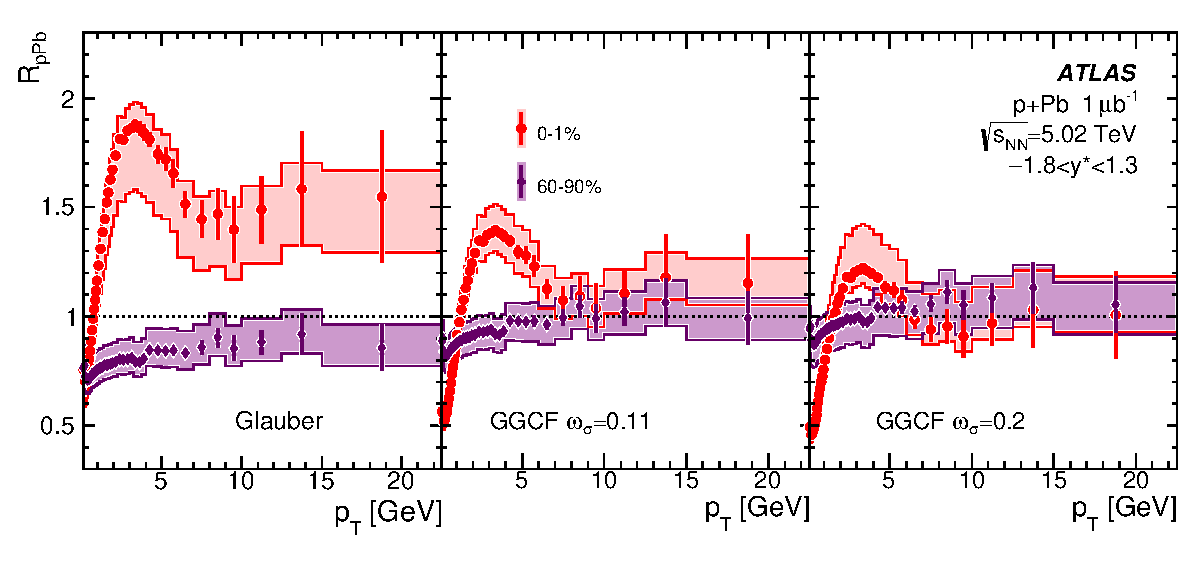
\includegraphics{rppb_cp.pdf}
  \caption{\RpPb for charged particles as a function of \pt for different collision geometries in the Glauber-Gribov color fluctuation model \cite{HION-2012-14}.}
  \label{fig:rppb_cp}
\end{figure}

A similar ratio is defined for \pA collisions.
\begin{equation}
  \RpA = \frac{\frac{1}{\Nevt}\frac{d N^{pA}_{X}}{d^3 p}}{\langle T_{pA} \rangle \frac{d\sigma^{pp}}{d^3 p}}
\end{equation}
For charged particles an apparent enhancement at high \pt can be explained by the \ac{GGCF} model \cite{HION-2012-14}, as shown in \cref{fig:rppb_cp}.
There is a sign of rapidity-dependent jet suppression in central \pPb collisions \cite{HION-2013-08}, although this is not a smoking gun for any medium formation because \RpPb is sensitive to other production effects like modifications to the nuclear \ac{PDF}.


\FloatBarrier
\subsubsection{Soft sector}

Particle production in high energy collisions is often decomposed into azimuthal Fourier components \cite{Voloshin:1994mz,Poskanzer:1998yz}. %% Heinz:2013th more recent summary
\begin{equation}
  \label{eq:flow_coefficients}
  E \frac{d^3 N}{d^3 p} = \frac{1}{2\pi \pt} \frac{d^2 N}{d\pt \, dy}\left\{ 1 + \sum_{n=1}^{\infty} 2v_n \cos\left[n(\phi - \Psi_n) \right] \right\}
\end{equation}
The $v_n$ are called the $n$th-order flow coefficients and the $\Psi_n$ are the $n$th-order event plane.
Experimentally they are defined by the relation (without corrections)
\begin{equation}
v_n e^{in\Psi_n} = \sum_k w_k e^{in\phi_k}
\end{equation}
where $w_k$ weights the $k$th particle or calorimeter element and is typically the \pt or $E_\mathrm{T}$ of the component.
This provides a framework for testing the predictions of dynamical models that describe the evolution of the initial energy deposited in the collision to the final-state bulk of particles.
For instance, a non-interacting gas model predicts $\langle v_n \rangle = 0$ for $n \geq 2$, with nonzero flow coefficients only from fluctuations, and is ruled out for \AA, \pA, and \pp collisions.

Hydrodynamics is a simple model that only assumes the system can be described by a fluid field with four-velocity $u^\mu(x^\nu)$ and imposes conservation of the stress-energy tensor $T^{\mu\nu}$ and possibly other conserved charges. %%, such that $\nabla_\mu T^{\mu\nu} = 0$.
The input of hydrodynamics is the specification of $T^{\mu\nu}$ itself, which typically includes an \ac{EoS} and multiple free parameters.
\Cref{sec:hydro} discusses relativistic hydrodynamic theory in detail.
The signature feature of fluid dynamics is the fact that accelerations are driven by pressure gradients.
For instance, in an ideal conformal fluid in $d$ spacetime dimensions
\begin{equation}
\dot{\mathbf{u}} = - \frac{1}{d} \boldsymbol{\nabla} \ln p
\end{equation}
where $\mathbf{u}$ is the vector part of $u^\mu$ and $p$ is the pressure.
Thus the shape of the initial energy density has a significant effect on the final particle distribution in \cref{eq:flow_coefficients}, as the fluid is pushed from regions of large density to small.

For the fluid description to be valid, matter must be able to readily interact with nearby fluid.
If disturbances in the velocity and energy fields are not propagated to nearby locations then the smooth description of the fields breaks down.
This requires the mean free path \mfp to be small compared to the length scale that the system evolves over, or equivalently, that the viscosity is small.
The applicability of hydrodynamics is discussed in further detail in \cref{subsec:hydro_applicability}.

\begin{figure}[t]
  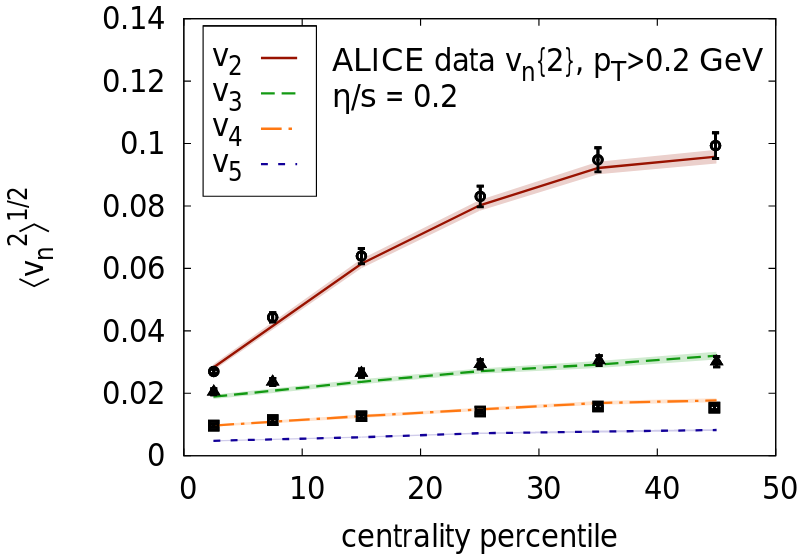
\includegraphics[width=0.49\linewidth]{vn_vs_cent.png}
  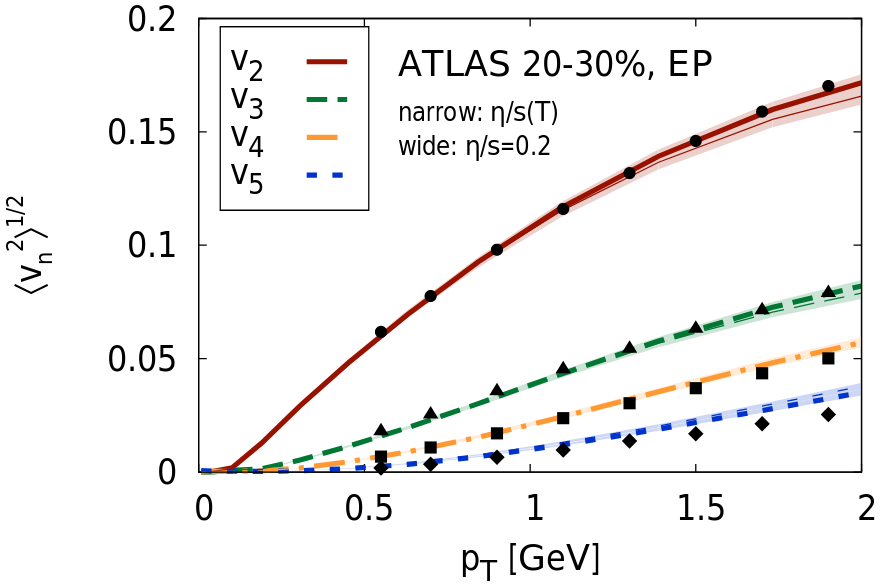
\includegraphics[width=0.49\linewidth]{vn_vs_pt.png}
  \caption{Event-by-event viscous hydrodynamic simulations of lead-lead collisions from \Ref{\cite{Gale:2012rq}} showing excellent agreement with experimental results as a function of centrality (left) \cite{ALICE:2011ab} and \pt (right) \cite{HION-2011-01}.}
  \label{fig:pbpb_vn}
\end{figure}

To a reasonable approximation, the 2nd- and 3rd-order flow coefficients are proportional to the corresponding eccentricities of the transverse source density \cite{Qiu:2011iv}, although $v_n$ for $n \geq 4$ include higher-order products.
The centrality of a \AA collision provides a control on the initial ellipticity, which is small for head-on central collisions with a circular transverse profile and larger for mid-central collisions with an almond-shaped overlap profile.
The $v_2$ as a function of centrality behaves according to this hydrodynamic prediction in \PbPb collisions.
Higher-order flow coefficients do not exhibit a strong centrality dependence because the higher-order eccentricities are not greatly dependent on the centrality.
The detailed simulations shown in \cref{fig:pbpb_vn} exhibit this behavior with excellent agreement with data as a function both of centrality and \pt.

Another key observation in \AuAu collisions is the scaling of the hadron flow coefficient with the hadron's number of constituent quarks $n_q$ \cite{Adare:2006ti}.
The hadron elliptic flow is found to scale with the kinetic energy such that $v_2^\textrm{hadron} = n_q v_2^\textrm{parton} \left(KT_\mathrm{T} / n_q\right)$.
This shows that the quarks themselves are indeed deconfined in the flow of the system, which amounts to strong evidence for the existence of the \qgp.

In \pp or \pA systems where the projectile has a radius that may be comparable to or smaller than the formation time, hydrodynamics is not na\"ively expected.
However, observations of a near-side azimuthal correlations in \pPb \cite{Abelev:2012ola,CMS-HIN-12-005,HION-2013-04} and \pp \cite{CMS-QCD-10-002,HION-2015-09} collisions show that these also exhibit collectivity, which is defined as pair correlations that arise not from direct interaction but from the global bulk evolution.
This ``ridge'' allows for the possibility of hydrodynamics in these smaller collisions, but hydrodynamics is not a necessary condition for collective behavior.
For instance, a \cgc model that invokes saturation of nuclear \acp{PDF} can predict a ridge in small systems with some success \cite{Dusling:2012cg,Dusling:2012wy,Dusling:2013qoz,McLerran:2013una,Kovchegov:2014yza}.

\begin{figure}[t]
  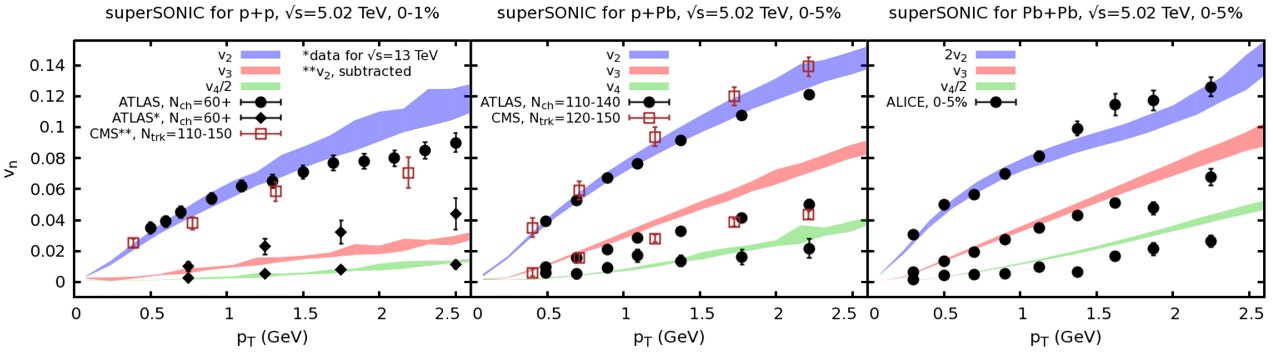
\includegraphics[width=\linewidth]{vn_all.png}
  \caption{Elliptic, triangular, and quadrupolar flow coefficients from superSONIC simulations (bands) compared to experimental data for proton-proton (left), proton-lead (center), and lead-lead (right) collisions \cite{Weller:2017tsr}. The specific viscosity parameters used in the simulations are $\eta/s = 0.08$ and $\zeta/s = 0.01$.}
  \label{fig:vn_all}
\end{figure}

Nevertheless, state-of-the-art viscous hydrodynamic simulations are capable of describing the flow coefficients in \pp, \pA, and \AA collisions simultaneously, as shown in \cref{fig:vn_all} \cite{Weller:2017tsr}.
Even in \pp collisions the $v_2$ seems to persist down to $\Nch \sim 20$ \cite{HION-2016-01}, however there is not yet complete agreement in the field over the experimental procedures used to extract the flow coefficients at very low \Nch.
For a review of hydrodynamics in small systems consult \Ref{\cite{Nagle:2018nvi}}.


\FloatBarrier
%% --------------------------------
%% Hydrodynamics
%% --------------------------------

\section{Hydrodynamic description of heavy ion collisions}
\label{sec:hydro}

\subsection{Relativistic fluid dynamics}

%% Poincar\'e instead of Lorentz?
Under the constraints of Lorentz symmetry and neglecting fluctuations, the stress-energy tensor of a perfect fluid described by flow four-velocity $u^\mu(x^\nu)$ is
\begin{equation}
%% T^{\mu\nu} = \left( \varepsilon + p \right) u^\mu u^\nu - p g^{\mu\nu} %% metric term has opposite sign for time-positive metric
T^{\mu\nu}_{(0)} = \varepsilon u^\mu u^\nu - p \Delta^{\mu\nu}
\end{equation}
where $\varepsilon$ and $p(\varepsilon)$ are respectively the energy density and pressure in the local rest frame.
The co-moving time-like and space-like projection operators are $u^\mu u^\nu$ and \( \Delta^{\mu\nu} \equiv g^{\mu\nu} - u^\mu u^\nu \), respectively.
In the absence of sources there are four conserved quantities corresponding to energy and three components of momentum.
\begin{equation}
  \label{eq:em_cons}
  \nabla_\mu T^{\mu\nu} = 0
\end{equation}
Projecting this equation into time and space components yields the relativistic Euler equations
\begin{align}
  D\varepsilon + \left(\varepsilon + p\right)\nabla^\perp_\mu u^\mu &= 0 \\
  \left(\varepsilon + p\right)Du^\mu + c_s^2 \nabla_\perp^\mu \varepsilon &= 0 
\end{align}
where \(D \equiv u^\mu \nabla_\mu\) is the co-moving time-like derivative, \( \nabla_\perp^\mu \equiv \Delta^{\mu\nu} \nabla_\nu \) is the co-moving space-like derivative, and \(c_s(\varepsilon) \equiv \sqrt{\frac{\partial p}{\partial \varepsilon}} \) can be identified with the speed of sound.
With a toy \ac{EoS} $p = c_s^2 \varepsilon$ the Euler equation is written as %% conformal/ultrarelativistic if c_s^2 = 1/3, e.g. photon gas
\begin{equation}
\dot{u}^\mu = \frac{c_s^2}{1+c_s^2} \frac{\nabla^\mu p}{p}
\end{equation}
which demonstrates that acceleration of the fluid is driven by pressure gradients.

The assumption of perfect fluidity is relaxed with the addition of the terms
\begin{equation}
T^{\mu\nu} = T^{\mu\nu}_{(0)} + \pi^{\mu\nu} + \Delta^{\mu\nu}\Pi
\end{equation}
where $\pi^{\mu\nu}$ and $\Pi$ are the shear stress and bulk stress that split the corrections into a traceless and trace part respectively.
To first order in gradients of $u^\mu$ and $\varepsilon$,
\begin{align}
  \label{eq:shear_stress}
  \pi^{\mu\nu} &= - \eta \sigma^{\mu\nu} \\
  \label{eq:bulk_stress}
  \Pi          &= - \zeta \nabla^\perp_\mu u^\mu
\end{align}
with
\begin{equation}
  \label{eq:sigma_tensor}
  \sigma^{\mu\nu} \equiv \nabla_\perp^\mu u^\nu + \nabla_\perp^\nu u^\mu - \frac{2}{3} \Delta^{\mu\nu}\nabla^\perp_\alpha u^\alpha \; ,
\end{equation}
and $\eta$ and $\zeta$ are the first order \emph{transport coefficients} which are called the shear viscosity and bulk viscosity, respectively.
Applying energy-momentum conservation (\cref{eq:em_cons}) with these 1st-order corrections yields the relativistic Navier-Stokes equations
\begin{align}
  D\varepsilon + \left(\varepsilon + p\right)\nabla^\perp_\mu u^\mu &= \frac{\eta}{2}\sigma^{\mu\nu}\sigma_{\mu\nu} + \zeta \left( \nabla^\perp_\mu u^\mu \right)^2 \\
  \left(\varepsilon + p\right)Du^\mu + c_s^2 \nabla_\perp^\mu \varepsilon &= \Delta^\mu_\beta \nabla_\alpha \left( \eta \sigma^{\alpha\beta} + \zeta \Delta^{\alpha\beta} \nabla^\perp_\nu u^\nu \right) \;,
\end{align}
but these equations violate causality by instantaneously propagating gradients to viscous stresses.
This causes instabilities in the solutions to these equations.
Causality can be recovered by expanding to second-order in the gradients \cite{Israel:1976tn} at the cost of introducing 15 second-order transport coefficients, four of which vanish in flat spacetime.
State-of-the-art simulations of the \qgp rely on second-order relativistic hydrodynamics \cite{Israel:1979wp}, though in practical applications many second-order coefficients are still fixed to zero.
In the conformal limit, for instance, $\zeta \rightarrow 0$ and there are five nonzero second-order transport coefficients \cite{Baier:2007ix,Marrochio:2013wla}.

\subsection{Applicability of hydrodynamics}
\label{subsec:hydro_applicability}

%% todo: possibly flesh this section out more?
%% dN/d\eta / \Npart \propto s^0.15 in AA and s^0.11 in pp (\sqrt{s}^0.3; \sqrt{s}^0.22) \cite{Aamodt:2010pb}
%% strongly-coupled: small eta/s ; weakly coupled gas: large eta
%% \todo{e.g. wavelength or \mfp < L}
%% eta \propto \varepsilon*\mfp from relativistic kinetic theory:
%%%    \eta \propto \rho\mfp<v> with \rho -> \varepsilon and <v> -> c
%% \mfp \propto 1/(n*\sigma) \propto 1/(s*\sigma)
%% also can have \mfp \propto eta/p with kinetic argument
%% \eta/s \propto T*\mfp
%% smaller \mfp means fluid element cannot traverse perpendicular to transfer momentum

%% low viscosity: large cross-section, low mfp

In order for hydrodynamics to be capable of a valid description, additional terms in the expansion of $T^{\mu\nu}$ must be small compared to existing terms.
The magnitude of the $\sigma^{\mu\nu}$ gradients in \cref{eq:sigma_tensor} can be estimated by the inverse system size $L^{-1}$.
The 1st-order term must be small compared to the 0th-order term, so a condition for the validity of hydrodynamics is \cite{Romatschke:2017ejr} %% eta/(ep+p) from arxiv:1712.05815 pg. 28
\begin{equation}
  \frac{\eta}{(\varepsilon + p)L} \ll 1 \;.
\end{equation}
With the approximation that the mean free path is \(\mfp = \frac{\eta}{\varepsilon + p} \), the condition is expressed in terms of the Knudsen number
\begin{equation}
  \mathrm{Kn} \equiv \frac{\mfp}{L} \ll 1 \;.
\end{equation}

The series produced in the hydrodynamic gradient expansion is not strictly convergent \cite{Denicol:2016bjh}.
This is because the number of terms grows like the factorial of the order of the expansion, and there is no lucky magic that exponentially suppresses the magnitude of the transport coefficients.
The Knudsen number in heavy ion simulations is not typically orders of magnitudes below unity \cite{Niemi:2014wta}; however, low-order viscous hydrodynamics has had ``unreasonable success'' at describing many global properties of heavy ion collisions.

Recent work has shown that the hydrodynamic expansion can be Borel-resummed \cite{Romatschke:2016hle,Romatschke:2017vte}, a method that produces an analytic continuation of the series.
The stress-energy tensor is split into a hydrodynamic attractor and a non-hydrodynamic component, with the cost that the transport coefficients become explicit functions of $\varepsilon$ and the gradients of $\varepsilon$ and $u^\mu$.
In this framework the condition for the applicability of hydrodynamics is weakened from thermal equilibrium to the requirement that these non-hydro modes are negligible.
%% The condition for the applicability of hydrodynamics is weakened from thermal equilibrium to the statement that these non-hydro modes are negligible.
In many examples it appears that the non-hydro modes decrease exponentially quickly, which potentially explains the ``unreasonable success'' of viscous hydrodynamics.
This also helps to explain the observations of some hydro-like phenomena in \pPb and even \pp collisions, where the small system size results in Knudsen numbers that are often greater than unity.


\subsection{Transport coefficients of the QGP} %% was titled ``and the AdS/CFT correspondence''

Hydrodynamics provides the framework for describing the bulk motion of fluid matter but is not capable of an independent determination of the \ac{EoS} or the transport coefficients.
Assumptions or results from microscopic theory are required to say anything about these quantities.
The \qcd \ac{EoS} is under control from lattice calculations, as discussed in \cref{subsec:lattice}. %% need to number subsections to have proper section number reference.

%% kinetic theory: $\eta/s = \tau_R T / 5$ where \tau_R is the relaxation time
At high temperatures the typical momentum is large, so the coupling is weak and perturbative calculations might be expected to apply.
To \ac{LO} the \ac{pQCD} shear viscosity is \cite{Arnold:2000dr}
\begin{equation}
\eta \propto \frac{T^3}{\alpha_s^2 \ln \left( 1/\alpha_s\right) }
\end{equation}
with a constant of proportionality dependent on the number of active quark flavors.
Perturbative calculations of the bulk viscosity at high temperature show that \cite{Arnold:2006fz}
\begin{equation}
\zeta \propto \frac{\alpha_s^2 T^3}{\ln \left(1/\alpha_s\right)}
\end{equation}
to \ac{LO}.
The bulk viscosity is suppressed by four powers of $\alpha_s$ relative to the shear viscosity, and is expected to vanish for conformal theories and in both in the low and high temperature limits.
It is therefore often neglected in discussions of the \qgp viscosity, though it can be relevant near the transition temperature and can enhance the Fourier harmonics of the particle production \cite{Noronha-Hostler:2013gga}.

The entropy density $s = (\varepsilon + p)/T$ also scales with the cube of temperature, so the shear viscosity is often normalized by the entropy density to form the specific viscosity $\eta/s$.
In \ac{pQCD} the value of the specific viscosity is close to unity near the critical point.
The condition for the validity of hydrodynamics from the previous discussion can be expressed as
\begin{equation}
  \frac{\eta}{s} \ll LT \;,
\end{equation}
which supports the intuition that matter with a small specific viscosity is expected to behave like a perfect fluid.
A lower bound can be placed on the viscosity based on arguments from the uncertainty principle \cite{Danielewicz:1984ww} such that $\eta \gtrsim 2T^3$.
With the Stefan-Boltzmann entropy, a bound is placed on the specific viscosity
\begin{equation}
  \label{eq:eta_over_s_uncertainty}
  \frac{\eta}{s} \gtrsim 0.1 \; ,
\end{equation}
so a perfect fluid is understood as one with viscosity that is not zero but is at the lower bound.
The $\eta/s$ of the \qgp is expected to have a minimum near the critical temperature \cite{Csernai:2006zz}.

One of the most influential theoretical developments of the past few decades is the conjectured relationship between quantum gravity in an \ac{AdS} space and a strongly-coupled \ac{CFT} \cite{Maldacena:1997re}.
This so-called \emph{\ac{AdS}/\ac{CFT} correspondence} allows calculations in a non-perturbative \ac{CFT} to be replaced by an associated calculation in weakly-coupled gravity, and is one of the only methods available to complete analytic calculations in the completely non-perturbative region.
The calculation of the shear viscosity in the strongly-coupled conformal limit gives a bound of \cite{Kovtun:2004de}
\begin{equation}
  \frac{\eta}{s} \geq \frac{1}{4\pi} \approx 0.08
\end{equation}
which is remarkably close to the bound from the uncertainty principle in \cref{eq:eta_over_s_uncertainty}.
Similarly the bulk viscosity has a temperature-dependent limit \cite{Buchel:2007mf}
\begin{equation}
  \frac{\zeta}{\eta} \geq 2\left(\frac{1}{3} - c_s^2 \right)
\end{equation}
which is positive in a non-conformal theory and larger than the perturbative calculation suggests. %% $\zeta/\eta \approx 15(1/3 - c_s^2)^2 \sim \alpha_s^4$.
These bounds are not expected to be exact in \qcd because it does not have all the symmetries of the corresponding supersymmetric \ac{CFT}.

Experimental measurements of collective flow anisotropies have been used to extract an experimental value of $\eta/s \approx 0.2 \approx 2.5\frac{1}{4\pi}$ \cite{Heinz:2013th}.
Recent simulations using the Kubo relations on the lattice for pure glue also report $\eta/s \approx 0.2$ near the critical point \cite{Astrakhantsev:2017nrs}, with hints that it rises slowly with the temperature.
The \qgp is quite close to a perfect quantum fluid.


\section{Femtoscopy in heavy ion collisions}
%% see this talk for cartoons:
%% https://indico.cern.ch/event/766194/contributions/3260610/attachments/1777242/2889870/WWND_ykawa_fin.pdf

Space-time correlations between the photons are used in astronomy to measure the size of stellar light sources.
These \ac{HBT} correlations \cite{HanburyBrown:1954,HanburyBrown:1956} are a consequence of Bose-Einstein statistics and manifest as increased probability for two photons to arrive at two detectors at similar times.
The width of the correlation in time difference is inversely proportional to the size of the distant star.
This process is called \emph{second-order interferometry}, as it requires a decoherent source in contrast to the type of interferometry exhibited in a classic double-slit experiment.

The procedure can be adapted to the tiny sources encountered in hadronic collisions using correlations in relative momentum space \cite{Goldhaber:1960sf}.
Though Bose-Einstein interactions are the simplest to leverage, in principle any non-trivial interaction can be used to image the source density.
The term \emph{femtoscopy} is used to refer to any measurement that provides spatio-temporal information of a hadronic source.

The measured \emph{\ac{HBT} radii} represent the dimensions of a nuclear source at freeze-out after all interactions between a final-state particle and the bulk are finished.
They are therefore sensitive to predictions regarding hydrodynamic expansion of an initial state.
The results of femtoscopic measurements in \pPb systems are of significant interest because they can shed light on the extent to which hydrodynamics applies in such small systems.

\subsection{Imaging the source density function}
Momentum space correlation functions can be written out in terms of source density functions, as detailed in the review in \Ref{\cite{Lisa:2005dd}}.
Particles are emitted on a freeze-out hypersurface denoted by $\partial\Sigma$.
The generation and interactions of $n$ particles before this hypersurface is described by a source density function $s_n(p_1, x_1;\ldots; p_n, x_n)$ of outgoing particle momenta $p_i$ and initial spacetime coordinates $x_i$.
The hypersurface $\partial\Sigma$ is not a region where each particle is created, but rather the surface of final interaction of the emitted particles with the bulk.
Though $s_n$ is only integrated over $\partial\Sigma$, the interactions before freeze-out are swept into the definition of $s_n$.
For two particles the following is written out:
\begin{equation}
  \begin{split}
  C(p_a,p_b) &\equiv \frac{E_a E_b \frac{dN}{d^3 p_a \, d^3 p_b}}{E_a \frac{dN}{d^3 p_a} E_b \frac{dN}{d^3p_b}} 
  \\&= \frac{\iint_{\partial\Sigma} d^3 x_a \, d^3 x_b \, s_2 (p_a, x_a; p_b, x_b) \left| \braket{ p_a, p_b | x_a, x_b } \right|^2}{\int_{\partial\Sigma} d^3 x_a \, s_1 (p_a, x_a) \, \int_{\partial\Sigma} d^3 x_b \, s_1(p_b, x_b)}
  \end{split}
\end{equation}
The "smoothness approximation" is typically invoked to approximate $\mathbf{p}_a \approx \frac{m_a}{m_a+m_b} \mathbf{k}$.
It is then convenient to define a normalization of the two-particle source density.
%% (We will skip a detailed discussion of the domain of integration of the variable $r = x_a - x_b$ and the equal-time approximation - for more see \cite{Lisa:2005dd}.) %% todo: maybe actually explain this
This normalization $S_2$ of $s_2$ is defined as follows:
\begin{equation} S_{2, \mathbf{k}} (\mathbf{r}) \equiv \frac{\iint_{\partial\Sigma} d^3 x_a \, d^3 x_b \, s_2 \left(\frac{m_a}{m_a+m_b}\mathbf{k}, x_a; \frac{m_b}{m_a+m_b}\mathbf{k}, x_b\right) \, \delta^3(\mathbf{r} - \mathbf{x}_a + \mathbf{x}_b)}{\int_{\partial\Sigma} d^3 x_a \, s_1 \left(\frac{m_a}{m_a+m_b}\mathbf{k}, x_a\right) \, \int_{\partial\Sigma} d^3 x_b \, s_1\left(\frac{m_b}{m_a+m_b}\mathbf{k}, x_b\right)}\end{equation}
If the resonances and other higher-order effects are ignored or removed, one can make the approximation that $s_2 (p_a, x_a; p_b, x_b) \approx s_1(p_a, x_a) s_1(p_b, x_b)$ which imposes the normalization constraint $\int d^3 r \, S_{2,\mathbf{k}}(\mathbf{r}) = 1$.

%% The correlation function can now be written in a simple and suggestive form.
Assuming that the center-of-mass motion is irrelevant after emission, the overall phase $e^{i\mathbf{k}\cdot(\mathbf{x}_a+\mathbf{x}_b)}$ can be factored out of the wavefunction (as in the example of \cref{eq:free_particle_wavefunction}), leaving only the relative part.
\begin{equation} \label{eq:wavefunction_kernel}
C_\mathbf{k}(\mathbf{q}) - 1 = \int d^3 r \, S_{2,\mathbf{k}}(\mathbf{r}) \left(\left|\braket{\mathbf{q}|\mathbf{r}}\right|^2 - 1 \right)
\end{equation}
This shows that the wavefunction is a kernel that transforms the source density function into the final-state correlation function.
The wavefunction kernel is only non-zero for interacting particles such that $\left|\braket{\mathbf{q}|\mathbf{r}}\right| = 1$.
For identical bosons, the resolving power is particularly strong due to wavefunction symmetrization.
In the approximation that all particles of a given charge are pions, that they are created in a fully chaotic source, and that they have no final-state interactions, the wavefunctions are simple plane waves and the resulting enhancement is the Fourier transform of the source density:
\begin{equation}
  \begin{split}
    \label{eq:free_particle_wavefunction}
\braket{\mathbf{k},\mathbf{q} | \mathbf{x}_a,\mathbf{x}_b} &= \frac{1}{\sqrt{2}}\left(e^{i\mathbf{p}_a \cdot \mathbf{x}_a + i\mathbf{p}_b \cdot \mathbf{x}_b} + e^{i\mathbf{p}_b \cdot \mathbf{x}_a + i\mathbf{p}_a \cdot \mathbf{x}_b}\right)\\
&= \frac{1}{\sqrt{2}} e^{i\mathbf{k} \cdot (\mathbf{x}_a+ \mathbf{x}_b)}\left(e^{i\mathbf{q} \cdot (\mathbf{x}_a - \mathbf{x}_b)/2} + e^{- i\mathbf{q} \cdot (\mathbf{x}_a - \mathbf{x}_b)/2}\right)\\
&= \sqrt{2}  e^{i\mathbf{k} \cdot (\mathbf{x}_a+ \mathbf{x}_b)} \cos\left( \frac{\mathbf{q} \cdot \Delta\mathbf{x}}{2} \right)\\
  \end{split}
\end{equation}
Plugging this back into the expression for the correlation function yields
\begin{equation}
  \begin{split}
C_{\mathbf{k}}(\mathbf{q}) - 1 &= \int d^3 r \, S_{\pi\pi,\mathbf{k}}(\mathbf{r}) \cos\left(\mathbf{q}\cdot\mathbf{r}\right)
\\&= \mathcal{F}\left[{S}_{\pi\pi,\mathbf{k}}\right] (\mathbf{q})
  \end{split}
\end{equation}
with the integration variable $\mathbf{r} = \Delta\mathbf{x}$.

In principle, any two interacting particle species can be used to image the source density.
The stronger the interaction, the more powerful the kernel is at resolving the source.
Bose-Einstein interactions are especially useful in nuclear collisions due to their increasing strength at small separations and the relative abundance of pions.

Some fraction of pions come from decays, long-lived resonances, or coherent emission, and the source function must be correspondingly modified \cite{Bowler:1991vx,Sinyukov:1998fc}.
Pairs in which one or both pions do not come from the core should be considered non-interacting since they are generated far apart, and the momentum scale of any Bose-Einstein effects are under the momentum resolution of the detector.
If the fraction of pairs with pions that both originate from the core is parameterized by $\lambda$, the source function in \cref{eq:wavefunction_kernel} should be expanded as
\begin{equation} S_{2}(r;\mathbf{k}) \rightarrow \lambda S_{2,\textrm{core}} (r;\mathbf{k}) + (1-\lambda) S_{2,\textrm{halo}} (r;\mathbf{k}) \end{equation}
where $S_c$ is the source function for pairs with both pions in the core and $S_h$ is the source for pairs involving the halo.
Pairs from the halo have a trivial wavefunction since they are effectively non-interacting.
For these the $\left(\left|\braket{\mathbf{q}|\mathbf{r}}\right|^2 - 1\right)$ term multiplying $S_h$ vanishes, and the correlation function becomes (hereafter we suppress some labels and understand $S$ to be the two-particle source function of the core)
\begin{equation}
  \begin{split}
    C_\mathbf{k}(\mathbf{q}) &= 1 + \lambda \int d^3 r \, S_{\mathbf{k}}(\mathbf{r}) \left(\left|\braket{\mathbf{q}|\mathbf{r}}\right|^2 - 1 \right)\\
    &= (1-\lambda) + \lambda \int d^3 r \, S_{\mathbf{k}}(\mathbf{r}) \left|\braket{\mathbf{q}|\mathbf{r}}\right|^2\\
    &= (1-\lambda) + \lambda \int d^3 r \, S_{\mathbf{k}}(\mathbf{r}) K(\mathbf{q},\mathbf{r}) \left(1 + \eta \cos\left(\mathbf{q}\cdot\mathbf{r}\right)\right)
  \end{split}
\end{equation}
where we have written the wavefunction as $\braket{\mathbf{q}|\mathbf{r}} = \sqrt{K(\mathbf{q},\mathbf{r})} \braket{\mathbf{q}|\mathbf{r}}_{\textrm{free}}$, with $K$ representing corrections to the free particle wavefunction, and where $\eta$ is the spin factor such that $\eta = \pm 1$ for bosons/fermions and $0$ for non-identical particles.
For instance, $K(\mathbf{q}) = G(\qinv)$ where $G(\qinv)$ is the Gamow factor accounts for Coulomb interactions between the final-state pions.
It is convenient to allow $K$ to be a function only of $q$, thus factoring it out of the integral.
This approximation is reasonable so long as the size of the source is small compared to the characteristic interaction length of the pair.
The particular choice for $K$, which includes a correction for the non-zero source size, is discussed in \cref{subsec:coulomb}.
With this simplification the correlation function can be expressed in a fairly general form as a function of the Fourier transform of the pair source density.
\begin{equation}
  \label{eq:correlation_function}
  C_\mathbf{k}(\mathbf{q}) = (1-\lambda) + \lambda K(\mathbf{q})\left\{ 1 + \eta \mathcal{F} \left[ S_\mathbf{k} \right](\mathbf{q}) \right\}
\end{equation}


\subsection{Parameterization of the correlation function}
\Cref{eq:correlation_function} relates an experimentally measured correlation function to the description of the source function encoded in its Fourier transform $\mathcal{F}[S_\mathbf{k}](\mathbf{q})$.
Extracting the source function $S_\mathbf{k}(\mathbf{r})$ directly from $C(q)$ by attempting to invert the Fourier integral transform $\mathcal{F}$ is impractical due to the noise in the measured correlation function.
\todo{here}

\subsubsection{L\'evy parameter}

%% A choice must be made to parameterize the description of $\mathcal{F}[S_\mathbf{k}]$.
When a generalization of the central limit theorem is considered, for which the requirement for finite variance is relaxed, one can derive the L\'evy-stable distributions \cite{Csorgo:2003uv}.
Their characteristic functions\footnote{i.e. Fourier transforms} are stretched exponentials, which are able to be expressed in terms of elementary functions and thus lend themselves readily to fitting.
In the approximation of ellipsoidal symmetry of the source, the Bose-Einstein part of the identical-pion correlation function can then be expressed as
\begin{equation} C_{\textrm{BE}}(\mathbf{q}) = 1 + \mathcal{F}[S_\mathbf{k}](\mathbf{q}) = 1 + e^{- \left\lVert R \mathbf{q} \right\rVert^{\alpha} } \end{equation}
where $R$ is a symmetric matrix whose components are the \ac{HBT} radii.
The L\'evy parameter $\alpha$ determines the tail weight of the underlying source density - the lower it is, the heavier the tails are.
Two particular cases are worth noting.
If $\alpha = 2$, the correlation function is a Gaussian and so is the source density, which is proportional to \( \exp\left(-\frac{1}{2} \mathbf{x} R^{-2} \mathbf{x}\right) \).
If $\alpha = 1$ the correlation function is a generalized exponential and the source density is Cauchy, proportional to \( \left( 1 + \mathbf{x} R^{-2} \mathbf{x} \right)^{-1} \).
It is common practice to fix $\alpha$ to one of these two values\footnote{The source densities corresponding to these stable functions have infinite variance if $\alpha < 2$, but the positive moments of the stable function itself are finite.
In $d$ spatial dimensions, the normalized $n^\textrm{th}$ $|q|$-moment of the correlation function's enhancement is given by
\begin{equation}
\left< q^n \right>_{\alpha} = \frac{\Gamma\left(\frac{n+d}{\alpha}\right)}{R^n \Gamma\left(\frac{d}{\alpha}\right)} \; .
\end{equation}
If it is assumed that the 1st moment was preserved under a fit (an assumption with validity depending heavily on the shape of the measured correlation function), the fit parameters measured at one choice of $\alpha$ could be related to those at another choice of $\alpha$, for instance $\Rinv^{\textrm{exp}} \sim \sqrt{\pi} \Rinv^{\textrm{gauss}}$.
This relation is sometimes used in the literature but it lacks rigorous motivation or support.}.
For the ATLAS \pPb results $\alpha$ is fixed to 1 because this choice has good agreement with data.
In many other results $\alpha = 2$ is used as this choice tends to work particularly well in \AA collisions.

%% experimental definition of correlation function in \cref{\label{sec:corr_func}}

\subsubsection{Coordinate system}
\label{subsubsec:coordinate}
In three dimensions a \ac{LCMF} is used, which is boosted to the longitudinal rest-frame of each pair of particles.
The coordinate axes are the Bertsch-Pratt coordinate system \cite{Pratt:1986cc,Bertsch:1989vn,Csorgo:1989kq}, which uses the ``out-side-long'' axes to separate the transverse part into components parallel (``out'') and perpendicular (``side'') to the pair's transverse momentum \kt.
\begin{align}
\qout &\equiv& \frac{\mathbf{k}_{\mathrm{T}} \cdot \mathbf{q}}{\left| \mathbf{k}_{\mathrm{T}} \right|}
&=& \frac{|\mathbf{p}^a_{\mathrm{T}}|^2 - |\mathbf{p}^b_{\mathrm{T}}|^2}{2 \kt}\\
\qside &\equiv& \frac{(\hat{\mathbf{z}} \times \mathbf{k}_{\mathrm{T}}) \cdot \mathbf{q}}{\left| \mathbf{k}_{\mathrm{T}} \right|} &=& - \frac{\hat{\mathbf{z}} \cdot \left(\mathbf{p}^a_{\mathrm{T}} \times \mathbf{p}^b_{\mathrm{T}}\right)}{\kt}\\
\qlong &\equiv& \hat{\mathbf{z}} \cdot \mathbf{q} &=& \frac{p^a_{z}E^{b} - p^b_{z}E^{a}}{\sqrt{k_{0}^2 - k_{z}^2}}
\end{align}
In a longitudinally-expanding hydrodynamic system this coordinate system is the local rest frame of the fluid elements.

\begin{figure}[t]
  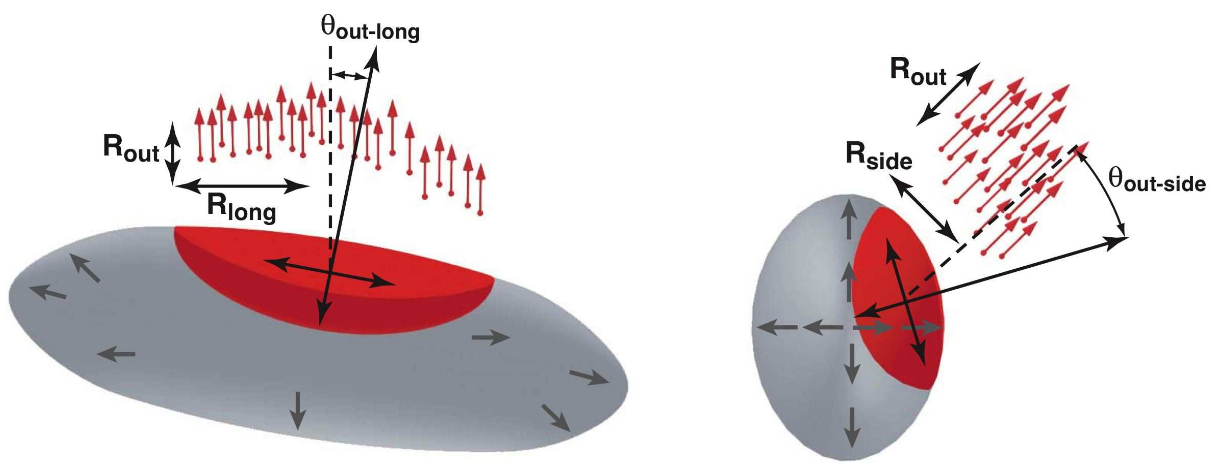
\includegraphics{hbt_radii_outsidelong.png}
  \caption{The HBT radii in the Bertsch-Pratt coordinate system \cite{Lisa:2005dd}. The longitudinal radius \Rlong is evaluated in the frame boosted to the pair's longitudinal momentum. The outwards transverse radius \Rout is along the pair's transverse momentum, and \Rside is the other transverse component.}
  \label{fig:hbt_outsidelong}
\end{figure}

The full \ac{HBT} matrix is written out in this coordinate system as
\begin{equation}
  \label{eq:r_matrix_full}
  R = \left( \begin{array}{ccc}
  \Rout & \Ros & \Rol \\
  \Ros & \Rside & \Rsl \\
  \Rol & \Rsl & \Rlong
  \end{array} \right) \; .
\end{equation}
The main \ac{HBT} radii are the diagonal terms of this matrix, illustrated in \cref{fig:hbt_outsidelong}.
The outwards radius \Rout represents the radial depth of the region of homogeneity as seen by the pair.
In hydrodynamic models the value of \Rout depends on the transverse velocity and the lifetime of the source.
The sideways radius \Rside is the transverse size of the source in the direction perpendicular to \kt.
The radius \Rlong indicates the longitudinal size of the region of homogeneity in the \ac{LCMF}.
Cross-terms \Ros, \Rol, and \Rsl are small relative to the main radii and in certain inclusive cases symmetries fix some or all of them to zero.

For identical particles the correlation function is symmetric under exchange of the pair, \(C(-\mathbf{q}) = C(\mathbf{q})\), so a single component of $\mathbf{q}$ can always be chosen as positive.
The order of a particle pair is picked such that $\qout > 0$.
Aside from the azimuthally-dependent results, the average azimuthal symmetry of the \pPb system is invoked so that $C(-\qside) = C(\qside)$, and it will be sufficient to consider only the absolute value $|\qside|$ and $\Ros = 0$.
In the azimuthally-dependent results, the \Rol term is sub-dominant compared to the other components\footnote{as shown in the results} and is fixed to zero, and only the absolute value of \qlong is considered.
In both cases $\Rsl = 0$.
In summary, for rapidity-dependent results only the \Rol cross-term is used
\[
R = \left( \begin{array}{ccc}
  \Rout & 0 & \Rol \\
  0 & \Rside & 0 \\
  \Rol & 0 & \Rlong
\end{array} \right) \;,
\]
and for the azimuthally-dependent results only \Ros is non-zero, with
\[
R = \left( \begin{array}{ccc}
  \Rout & \Ros & 0 \\
  \Ros & \Rside & 0 \\
  0 & 0 & \Rlong
\end{array} \right) \; .
\]

Motivated by the Gaussian parameterization\footnote{i.e. the L\'evy parameter $\alpha = 2$}, many results report the square of the matrix $R^2$ rather than the $R$ matrix defined here with units of length.
This must be accounted for when comparing results using different conventions.
Fortunately a comparison is simple when the cross-terms are relatively small, as
\begin{equation}
  R^2 = \left( \begin{array}{ccc}
  \Rout^2 & \Ros(\Rout+\Rside) & \Rol(\Rout+\Rlong) \\
  \Ros(\Rout+\Rside) & \Rside^2 & 0 \\
  \Rol(\Rout+\Rlong) & 0 & \Rlong^2
  \end{array} \right) + \bigo{ \Ros^2, \Rol^2, \Ros \Rol }
\end{equation}
with $\Rsl = 0$.

\subsection{HBT radii under collective flow}

The femtoscopic radii are not equivalent to the total size of the source but rather indicate the size of the region of homogeneity.
This volume is the effective size of the source with which particles have equilibrium.
Collective expansion makes it more difficult for two regions of the source to equilibrate as they are pushed apart from each other.
In an infinite volume the size of the region of homogeneity is set by the length scale at which collective velocity overcomes thermal velocity \cite{Lisa:2005dd} so
\begin{equation}
R_i \sim \frac{v_\textrm{thermal}}{\frac{du}{dx_i}}
\end{equation}
where the collective velocity is described by the function $u(x)$.

\begin{figure}[t]
  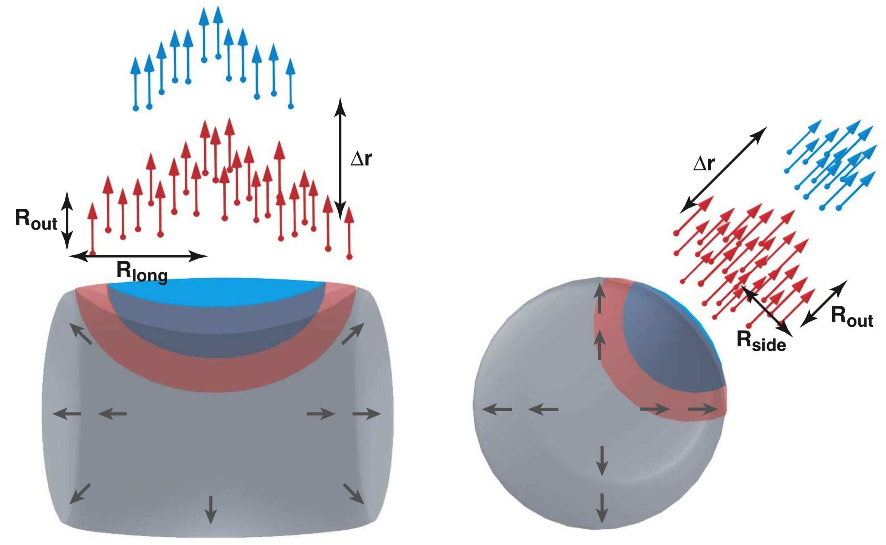
\includegraphics{hbt_radii_flow.png}
  \caption{Particles with a higher \pt give smaller values of \Rlong under longitudinal flow (left) and smaller values of the transverse radii under radial flow (right) \cite{Lisa:2005dd}.}
  \label{fig:hbt_flow}
\end{figure}

After a heavy ion collision the generated matter is spread longitudinally between the nuclear remnants with boundaries traveling away from the \ac{IP} at speed $c$.
The collective velocity profile is approximated as $u = z/t$ in the absence of longitudinal acceleration.
The longitudinal radius is then determined by the expected emission time
\begin{equation}
  \Rlong \approx v_\textrm{thermal} \langle t \rangle \; .
\end{equation}
The thermal velocity scales with $\sqrt{T/\mt}$ at large \mt where $\mt = \sqrt{m^2 + \pt^2}$ is the transverse mass.
However, because particles with larger \mt are typically emitted earlier, \Rlong may be expected to decrease more rapidly than $1/\sqrt{\mt}$.

Transverse expansion is generated by the particular dynamics of the system, so the dependence of the transverse radii on \mt depends on the choice of blast wave model.
Generally a similar decrease with \mt is predicted for \Rout and \Rside as well as \Rlong, as shown in \cref{fig:hbt_flow}. Generally the decrease of femtoscopic radii with rising pair \kt is interpreted as a signature of collective expansion \cite{Kolb:2003dz}.

%% \cite{Kolehmainen:1986fe,Padula:1989ie} %% bjorken flow correlation function


\subsection{Motivation for femtoscopy in proton-lead collisions}
Femtoscopic measurements have already been made in \pPb collisions \cite{Abelev:2014pja,Adam:2015pya} but there is space for advancement.
The \kt-dependence of these measured \ac{HBT} radii suggests collective expansion even in peripheral collisions.
However, this pattern is faked by the increasing relevance of jet fragmentation correlations at larger \kt and in peripheral collisions, and the method used to account for this background is susceptible to this bias.
Thus increasing sophistication in the methods used to constrain this background are desirable.
In addition, rapidity-dependent measurements of the radii have the potential to have nontrivial behavior in an asymmetric \pA system, and ATLAS is particularly well-suited to such a measurement with an inner detector covering 5 units of pseudorapidity.

Because femtoscopy provides a measurement of the source's spatial dimensions, it is particularly useful for probing the hydrodynamic prediction that spatial anisotropies lead to complementary momentum anisotropies.
Elliptic modulation of the freeze-out shape has been observed in \AuAu \cite{Adams:2003ra,Adare:2014vax,Adamczyk:2014mxp} and \PbPb \cite{Adamova:2017opl} collisions.
These measurements show that the transverse radii are reduced along the event plane axis compared to out-of-plane.
The second-order Fourier coefficient of \Rside is shown in \cref{fig:rside_v2_aa} for \AuAu and \PbPb systems as a function of the initial ellipticity computed in the MC Glauber model.
The final source ellipticity, indicated by $\Rside{}_{,c2} / \Rside{}_{,0}$, has the same sign as the initial ellipticity but with a reduced magnitude.
This is consistent with an elliptic transverse source profile that expands more along the minor axis but not enough to overtake the length of the major axis.

\begin{figure}[t]
  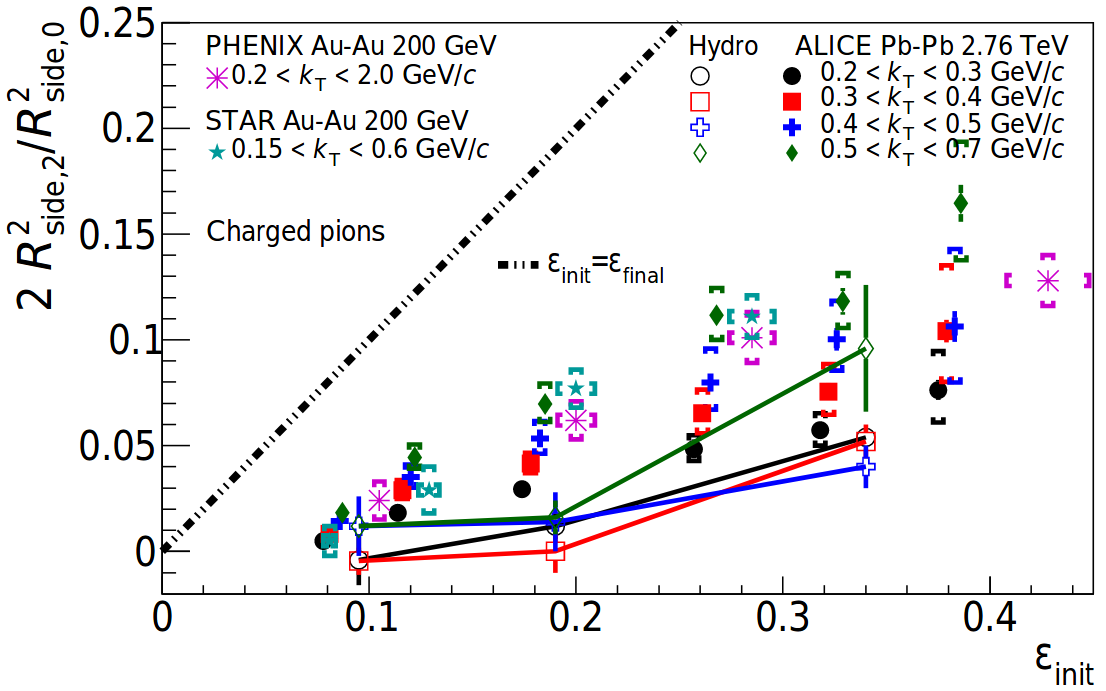
\includegraphics{azi_hbt_aa_ellipticity.png}
  \caption{The relative second-order Fourier coefficient of \Rside in nucleus-nucleus collisions compared to the initial source eccentricity calculated from the MC Glauber model \cite{Adamova:2017opl}.}
  \label{fig:rside_v2_aa}
\end{figure}

Azimuthal measurements are challenging outside of \AA collisions because the resolution of the event plane \psit depends heavily on the event activity.
ATLAS has a reasonably high event plane resolution in central \pPb events with reasonably large elliptic flow.
An observation of the same type of azimuthal dependence of the \ac{HBT} radii that is observed in \AA collisions would provide compelling evidence for the hydrodynamic behavior of central \pPb collisions.
